\documentclass{article}
\usepackage[utf8]{inputenc}
\usepackage{listings}
\usepackage{graphicx}
\usepackage{float}
\usepackage{enumitem}
\usepackage{hyperref}

\setlength{\parindent}{0pt}
\lstset{
    basicstyle=\ttfamily\footnotesize,
    frame=single,
    xleftmargin=4pt,
    xrightmargin=4pt,
    breaklines=true
}

\title{Cloud Temperature \& Humidity Notification System}
\author{Lue Xiong}

\begin{document}

\maketitle
\newpage

\tableofcontents
\newpage

\obeylines

\section{Context}
The Cloud Temperature \& Humidity Notification System is about an IoT system that gives the ability to notify users of temperature and humidity fluctuations within their living environment through the usage of a Simple Message Service, which is also known as SMS. The system will also notify a user if the Particle Argon is offline by checking that data is being sent and stored in the database. Though this is the main concern of the system, it also allows users to visualize their daily climate averages in an interactive graph. The graph is automatically updated for the users to view whenever they want to on the web. Behind the scenes, most computation is abstracted away from the user by using the Google Cloud Platform. The initiation of these functionalities start from the ambient temperature and relative humidity readings being published by the Particle Argon.\\

This system represents a single IoT device that performs the above-mentioned functionalities. One can imagine, however, being able to send in-home area location data and climate readings with a multiple of these IoT devices scattered across a home with multiple rooms and stories. A user would be notified where in the house and when the climate has reached configured threshold levels for each device. They would then be able to see data points for each specified area of the home. Ideally, aspects of the system such as climate data publishing intervals, setting climate threshold and maximum notification intervals, and timezones should be configurable. With that said, the project seeks a minimum viable product. That is, the system will notify users of climate thresholds being met and device status through SMS notification as well as graphing average climate per day for viewing averages over days. User configuration will be beyond the minimum viable product as it would require additional development of a web application.\\

Though the system is targeted for the home living environment, it can be used for environments that require careful monitoring. Take a fermented product like kombucha for instance; it needs to be fermented in an environment where the ambient temperature hovers in the range of 65 to 85 degrees Fahrenheit over a week to multiple weeks. Low temperatures will either stop or dramatically slow down the fermentation process. High temperatures will quicken the fermentation process but also increases the risk of unwanted bacteria or mold growth that would ruin the product. Striking a balance with temperature for optimal conditions is difficult without information. The usage is only limited to the imagination.\\

The Cloud Temperature \& Humidity Notification System source code can be found in GitHub linked here: \\

\url{https://github.com/lxiong1/cloud-temperature-humidity-notification}.

\section{Problem}
The problem trying to be solved is giving users climate data information about their living environment that they need to act on. Certain ranges of temperature and humidity affect humans in ways that are detrimental to their health. For example, low humidity environments --characterized as 30\% relative humidity and below -- is a condition for being prone to respiratory infections, dry eyes, and itchy irritated skin. High humidity environments -- characterized as 60\% and above -- is a condition for bacterial and mold growth, a catalyst for the decomposition of organic materials, and the attraction of bugs and insects to the home. A way to solve that problem is to give a renter or homeowner actionable data to understand that their living environment needs change. That is where the Cloud Temperature \& Humidity Notification System comes in.

\section{Market Research}
From market researching, there are a couple of products that have similar functionalities:

\begin{itemize}
	\setlength{\itemindent}{.3in}
	\item AcuRite 01152M 3-Sensor Indoor Monitoring
	\item Govee Temperature Humidity Monitor
	\item Proteus AMBIO
\end{itemize}

All three of these products measure temperature and humidity and have their value propositions. We'll briefly go through what they are and how they function. For differentiation between these products and the Cloud Temperature \& Humidity Notification System, please read through Section~\ref{section:overview} and~\ref{section:process}.

\subsection{AcuRite 01152M 3-Sensor Indoor Monitoring}
AcuRite 1166M is packaged with 3 sensor units along with what they call a \textit{smartHUB}. The name is self-explanatory, it is the central communication piece for the 3 sensors. The max connection capacity for the smartHUB is 7 sensors. This system use bluetooth technology to pair the sensors to the smartHUB using a mobile application with a distance limit of 330 feet between sensor and hub. These sensors will read in the climate information of the environment and send it over to the smartHUB, which will then send information over to the mobile application to be processed and viewed. There are some inherent flaws with this system as I will explain.\\

With the max capacity being 7 sensors connected to the smartHUB, it is only usable in a home environment and even then, a user may want more sensors if they have a larger home. The reason for the limitation is the design of having sensors centered around the smartHUB, and not standalone pieces. The sensors are nothing without the smartHUB, therefore renders the system useless if it breaks. It also adds one more layer of complexity that is unnecessary for the user because it is not doing anything complex enough to justify a central hub. This system is also all local-based, it does not support WiFi connections so a user has to be physically present in the home to understand be able tp update and view up-to-date climate data.\\

Another issue is reliability. The range at which these sensors can communicate with the smartHUB is limited and depending on the distance from sensor to hub, structure, materials, and size of the home can make it more difficult to reliably transfer information from sensor to hub. With a 3.5 star rating on Amazon and complaints of reliability-related issues, it's clear why this does not work all too well. The AcuRite 01152M on Amazon is linked here:\\

\url{https://www.amazon.com/AcuRite-01006M-Temperature-Monitoring-Compatible/dp/B07CBFMJQM/ref=sr_1_1?dchild=1&keywords=AcuRite\%2B01166M&qid=1588272832&sr=8-1&th=1}\\

That 3.5 star rating with 74 reviews cannot be trusted either. Fakespot -- a company that develops software to analyze reviews from retail shops -- puts the AcuRite 01152M reviews from the Amazon link above in a \textbf{D} grade as shown by Figure~\ref{fig:acurite}. That means that likely a lot of the reviews are fake. Fakespot estimates that 54.1\% of reviews are reliable.\\

\begin{figure}[H]
	\center
	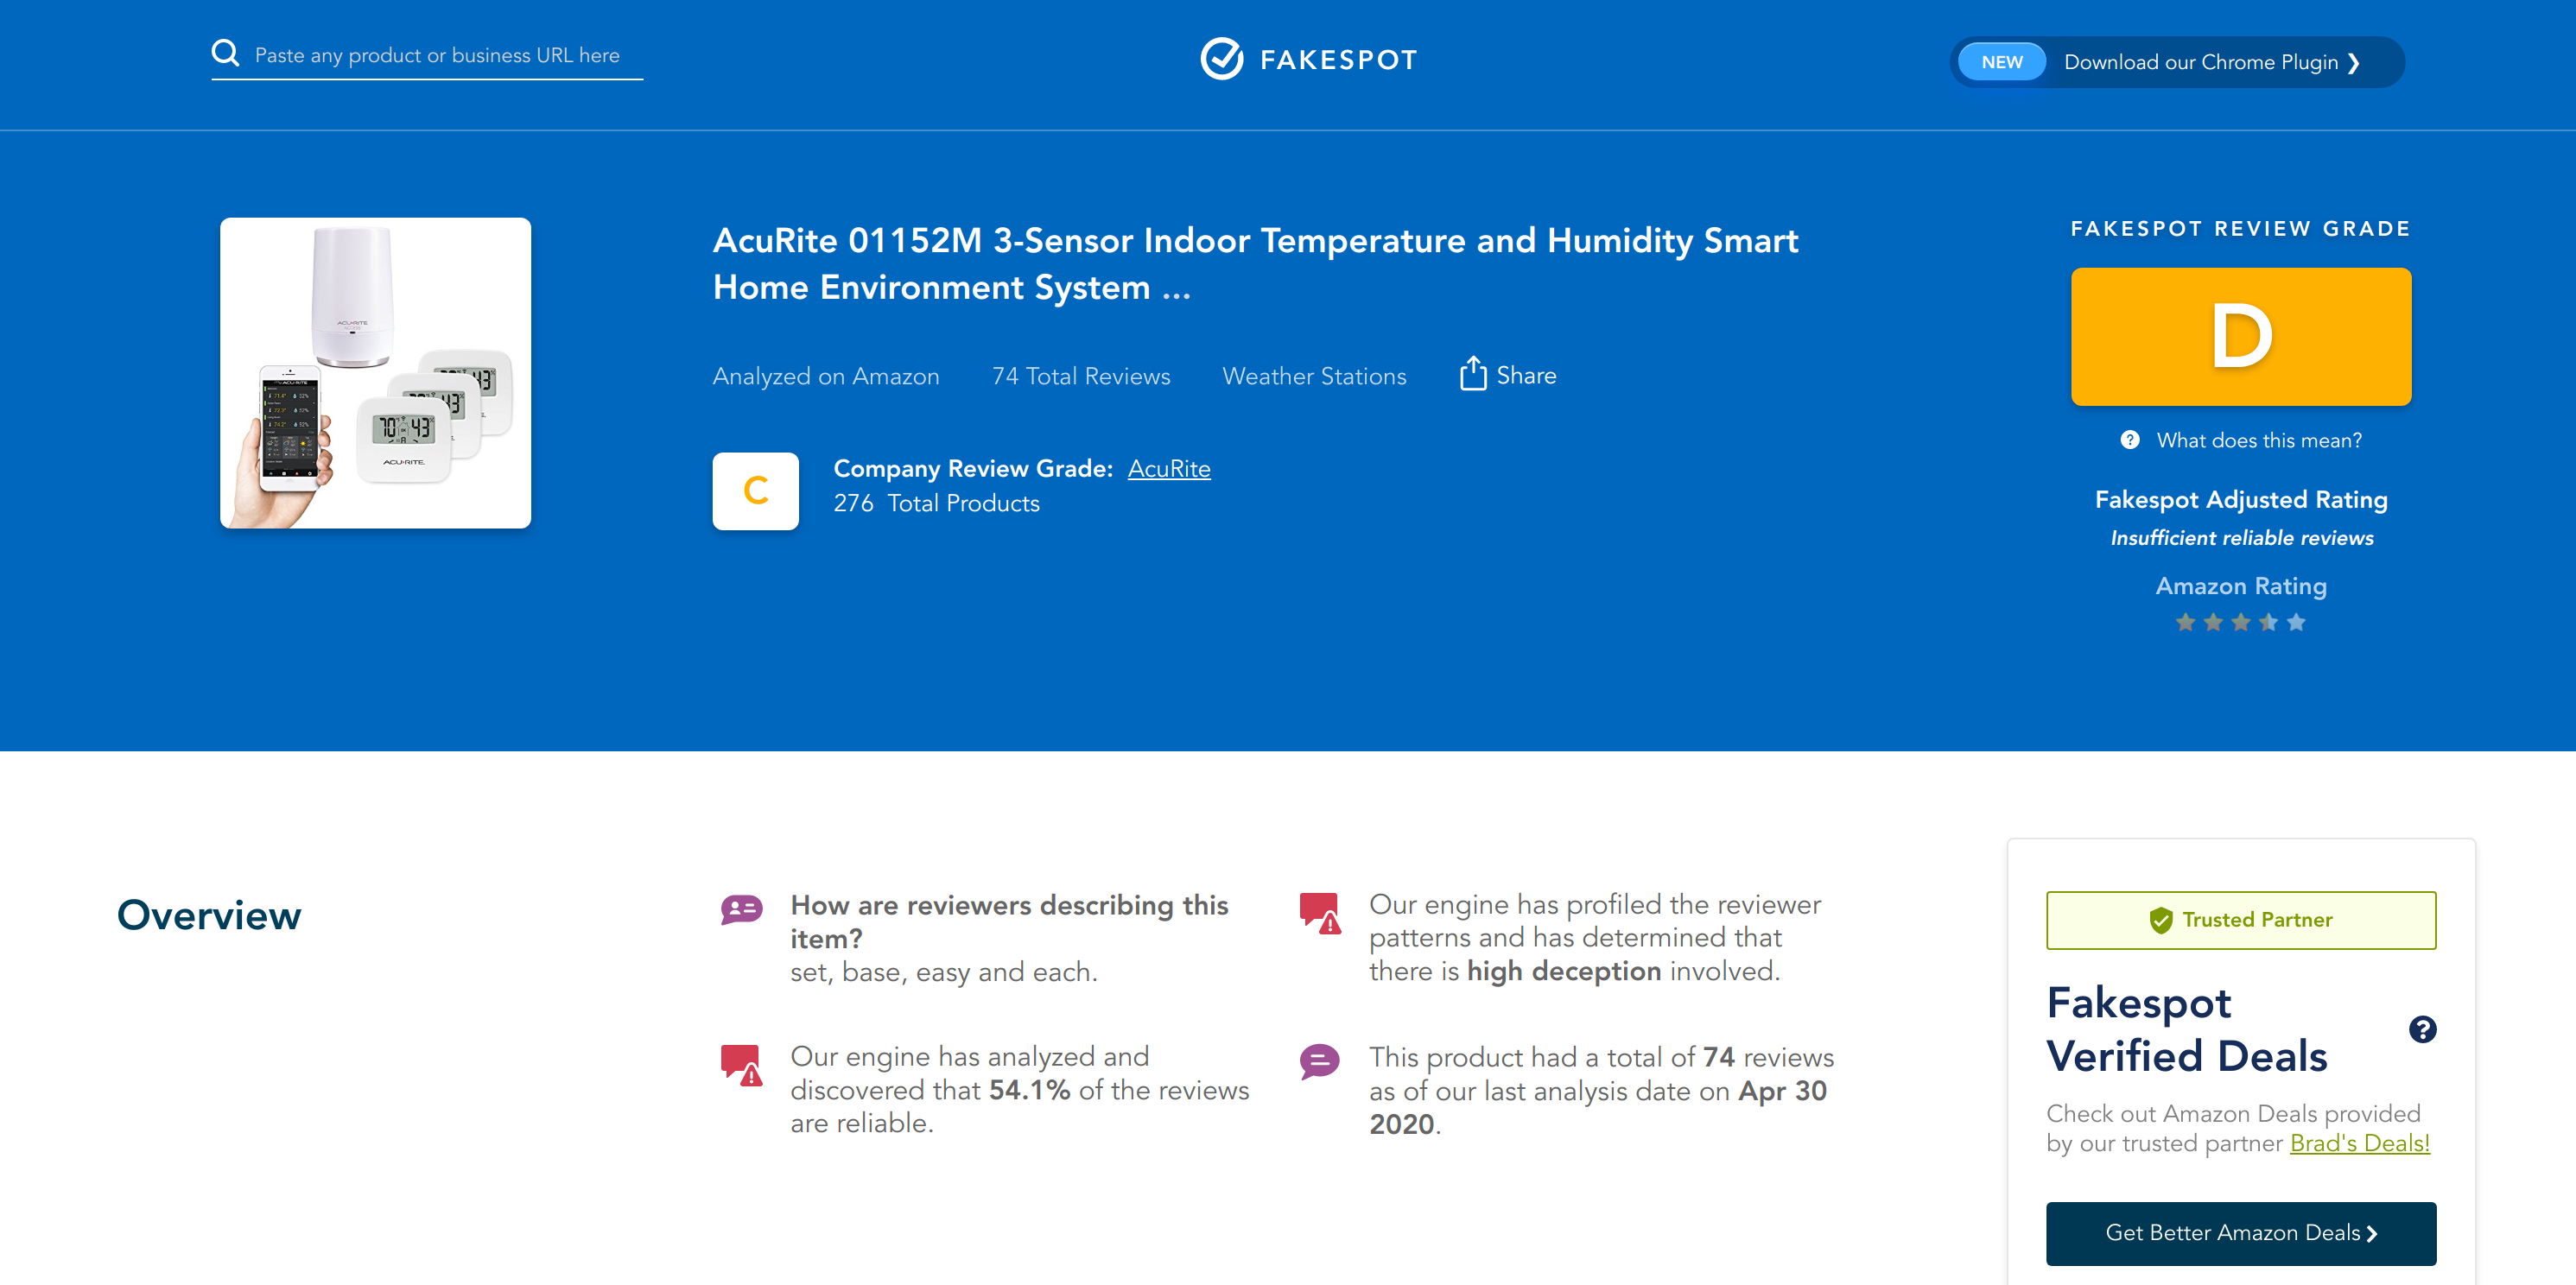
\includegraphics[width=\textwidth]{images/acurite-fakespot.png}
	\caption{Fakespot Grading of AcuRite 01152M}
	\label{fig:acurite}
\end{figure}

The last thing to point out is how expensive this setup is. The price for the 3 sensors and smartHUB is currently priced at \$124.07. That is a lot of money to spend on a system that is seemingly unreliable.

\subsection{Govee Temperature Humidity Monitor (WiFi Edition)}
The Govee Temperature Humidity Monitor has an LCD screen that displays temperature and humdity. It uses bluetooth technology to pair the product itself with a mobile application and has a distance limit of 330 feet. It also has the capability to connect to WiFi. Every 10 minutes, it will upload all climate data recorded on the paired smartphone within that timeframe. It also sends a push notification to the mobile application on a user-configured alert threshold.\\

\url{https://www.amazon.com/MINGER-Temperature-Humidity-Hygrometer-Thermometer/dp/B07FBCTQ3L/ref=sr_1_8?dchild=1&keywords=Govee+Temperature+Humidity+Monitor&qid=1588275020&sr=8-8}\\

\begin{figure}[H]
	\center
	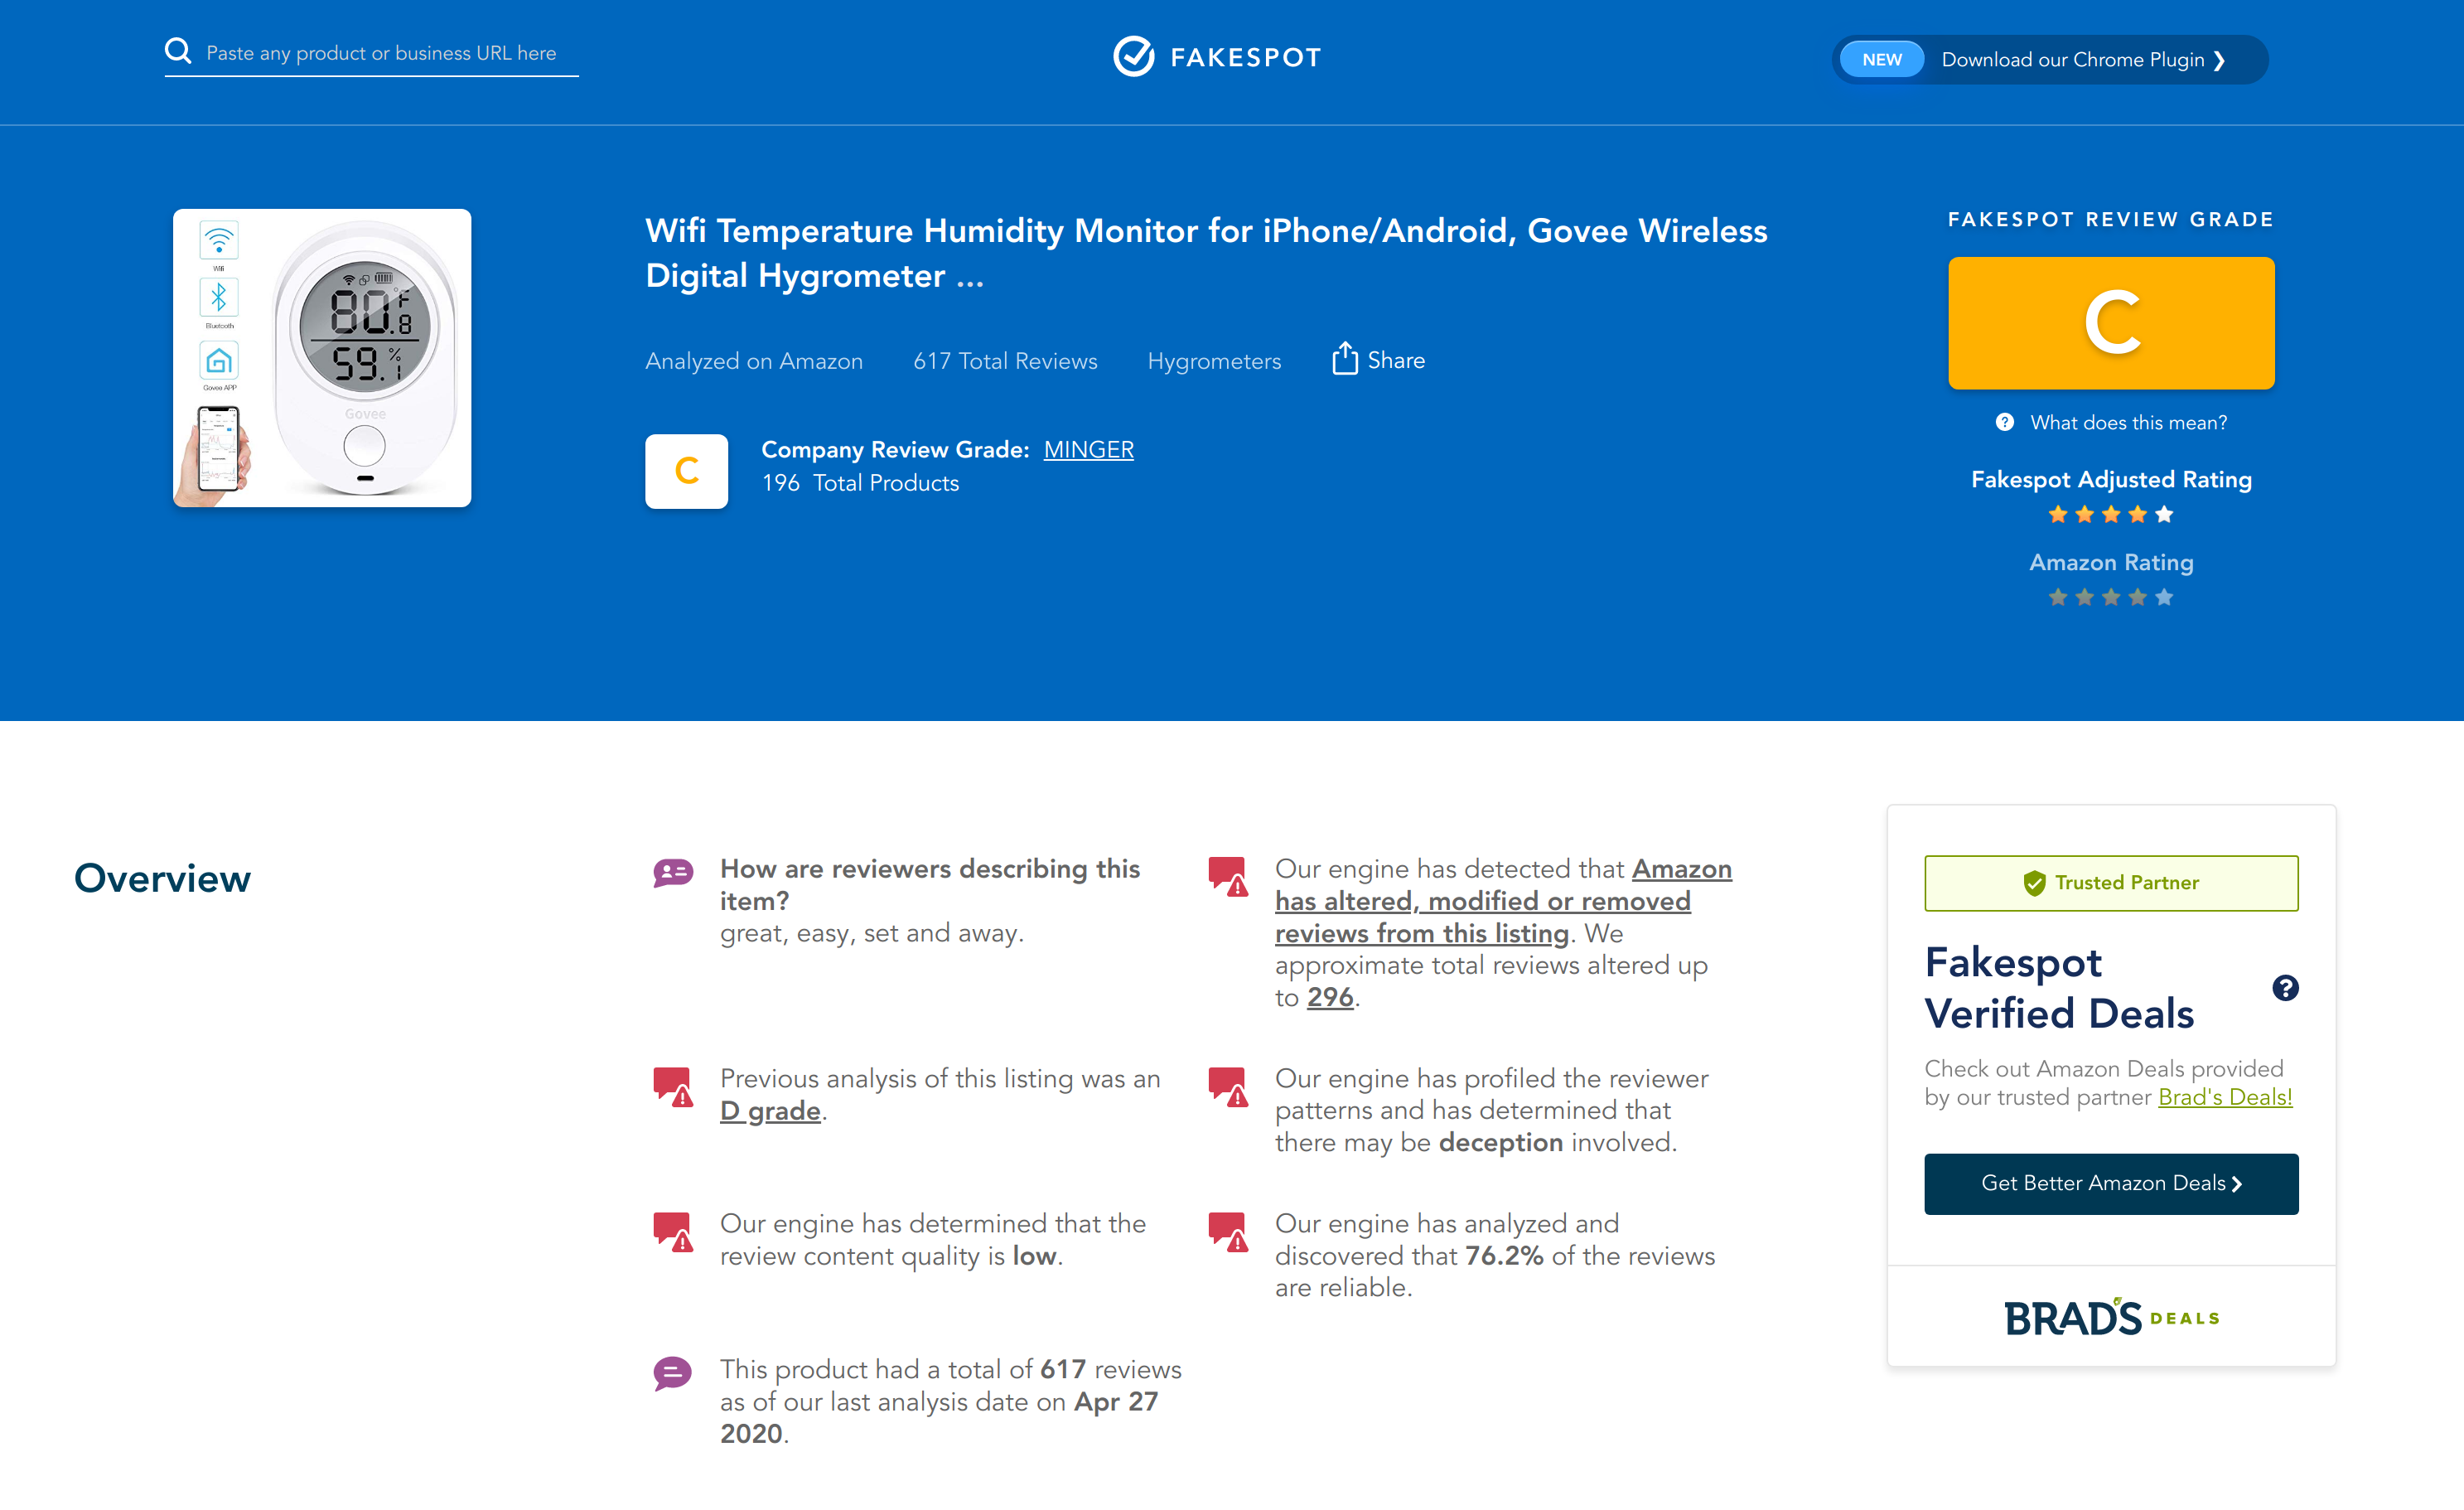
\includegraphics[width=\textwidth]{images/govee-fakespot.png}
	\caption{Fakespot Grading of Govee Temperature Humidity Monitor}
	\label{fig:govee}
\end{figure}

The Govee Temperature Humidity Monitor is rated at 4.1 stars with 618 reviews. Fakespot graded the Amazon reviews for the product at a C grade while estimating that 76.2\% of them are reliable as shown in Figure~\ref{fig:govee}. Not exactly a condfident rating. It is priced at \$49.99.

\subsection{Proteus AMBIO}
The Proteus AMBIO reads temperature and humidity data over the network and provides the ability to view climate data through a mobile application. To power on the device, it has to be plugged into an outlet. There no are subscription fees or monthly charges needed after purchasing the product.\\

\url{https://www.amazon.com/Temperature-Humidity-sensor-Buzzer-Alerts/dp/B01AQ0PZFS/ref=sr_1_2?dchild=1&keywords=Proteus+AMBIO&qid=1588276223&sr=8-2}\\

\begin{figure}[H]
	\center
	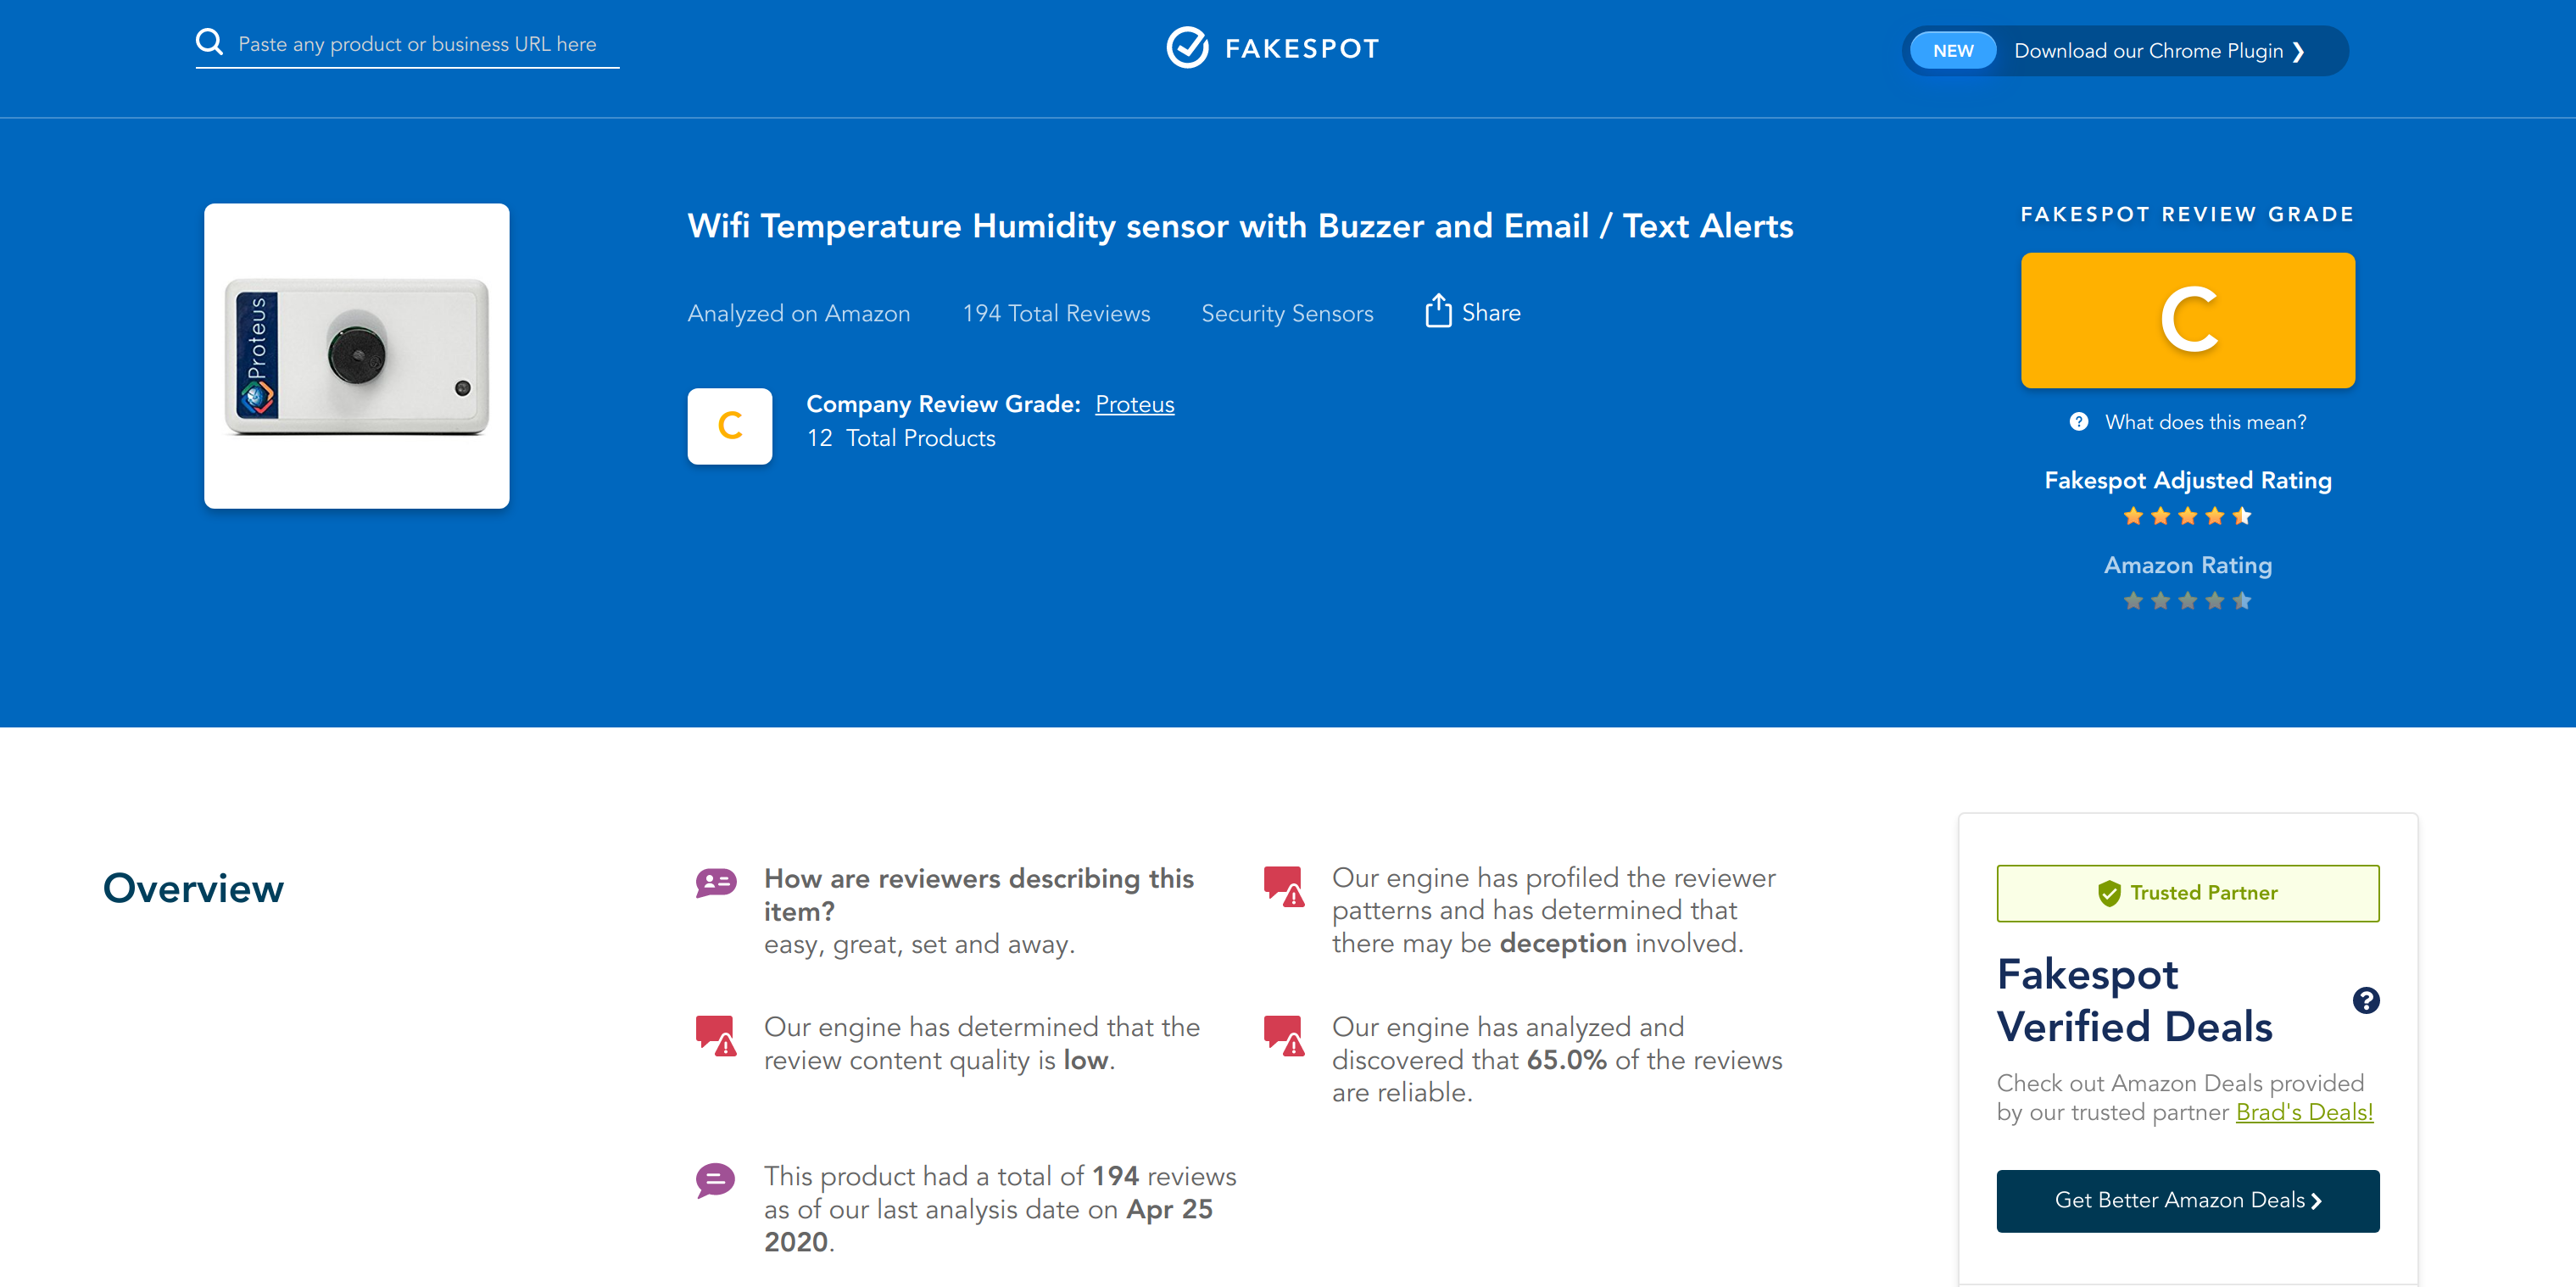
\includegraphics[width=\textwidth]{images/proteus-fakespot.png}
	\caption{Fakespot Grading of Proteus AMBIO}
	\label{fig:proteus}
\end{figure}

Proteus AMBIO is rated at 4.6 stars with 196 reviews. Fakespot graded the Amazon reviews for the product at a C grade while estimating that 65\% of them are reliable as shown in Figure~\ref{fig:proteus}. Again, Not exactly a condfident rating. It is priced at \$99.00.

\section{System Overview}
\label{section:overview}
This section will describe the minimum viable product requirements and the architectural decision made for achieving the desired results of the system.

\subsection{System Requirements}
To satisfy the need of giving a user useful information about temperature and humidity in their targeted environment, the following are the minimum viable product requirements:

\begin{itemize}
    \setlength{\itemindent}{.3in}
    \item Device shall be able to connect to WiFi
    \item Device shall be able to sense ambient temperature
    \item Device shall be able to sense relative humdiity
	\item All notifications sent to the user shall be an SMS message
	\item Notifications sent to the user shall be based on the following criteria
	      \begin{itemize}
		      \setlength{\itemindent}{.5in}
		      \item Temperature upper threshold shall be set to lesser than or equal to 75 degrees Fahrenheit
		      \item Temperature lower threshold shall be set to greater than or equal to 65 degrees Fahrenheit
		      \item Humidity upper threshold shall be set to lesser than or equal to 60 percent relative humidity
		      \item Humidity lower threshold shall be set to greater than or equal to 30 percent relative humidity
	      \end{itemize}
	\item Minimum 1-hour gap in between each SMS message per climate type (AKA temperature and humidity) reaching above or below the threshold value
	\item The status of the device publishing temperature and humidity data must be checked every hour
	      \begin{itemize}
		      \setlength{\itemindent}{.5in}
		      \item When the device is online, nothing shall happen
		      \item When the device is offline, the user shall be notified
	      \end{itemize}
	\item Working hours shall be defined as 6 AM to 9 PM CDT
	\item Device shall publish every 15 minutes during the working hours
	\item Device shall publish every 30 minutes during the non-working hours
	\item System shall create a daily graph aggregating temperature and humidity averages over days at 9 PM CDT
\end{itemize}

\subsection{Event-Driven Serverless Architecture}
\label{section:architecture}
The approach taken for the system as mentioned before is heavy on the software side and manifested into an event-driven serverless architecture. An event-driven serverless architecture in the system context allows the climate data readings to be sent as events, processed based on its event type, and have actions performed without the need for standing up servers. The following are benefits of the said architecture:

\begin{itemize}
	\setlength{\itemindent}{.3in}
	\item Loose coupling between software components
	\item Automatic scaling based on user demand
	\item All processing is driven by events
	\item No need for management of servers
	\item Overall cost reduction versus self-managed servers
	\item Inherent stateless nature
\end{itemize}

While these benefits are good to have, every architectural decision has its drawbacks. The following  are drawbacks of the said architecture:

\begin{itemize}
	\setlength{\itemindent}{.3in}
	\item Each serverless function must provide its own packaged dependencies
	\item Having a large number of serverless functions can become unwieldy
	\item Long-running processes are not fit for serverless functions
	\item Handling system state amongst stateless functions can be tricky
\end{itemize}

Using an event-driven serverless architecture made sense for this system, as the needs of the system are fulfilled automatically on publishing data without any manual intervention.

\section{Process and Implementation}
\label{section:process}
I will preface that the Cloud Temperature \& Humidity Notification System is heavily software-based. The hardware components are nothing special and ultimately serve as a vessel for sending climate information to be processed in the cloud to create the closed-feedback loop. The Particle Argon referenced in Section~\ref{section:hardware} will contain firmware that is fundamental to the system requirements and architectural decision in Section~\ref{section:overview}. This particular section will describe the thought process behind the implementation, considerations taken during development, and how the system performs user notification and automatic graph updates.

\subsection{Hardware Components}
\label{section:hardware}
\begin{figure}[H]
	\center
	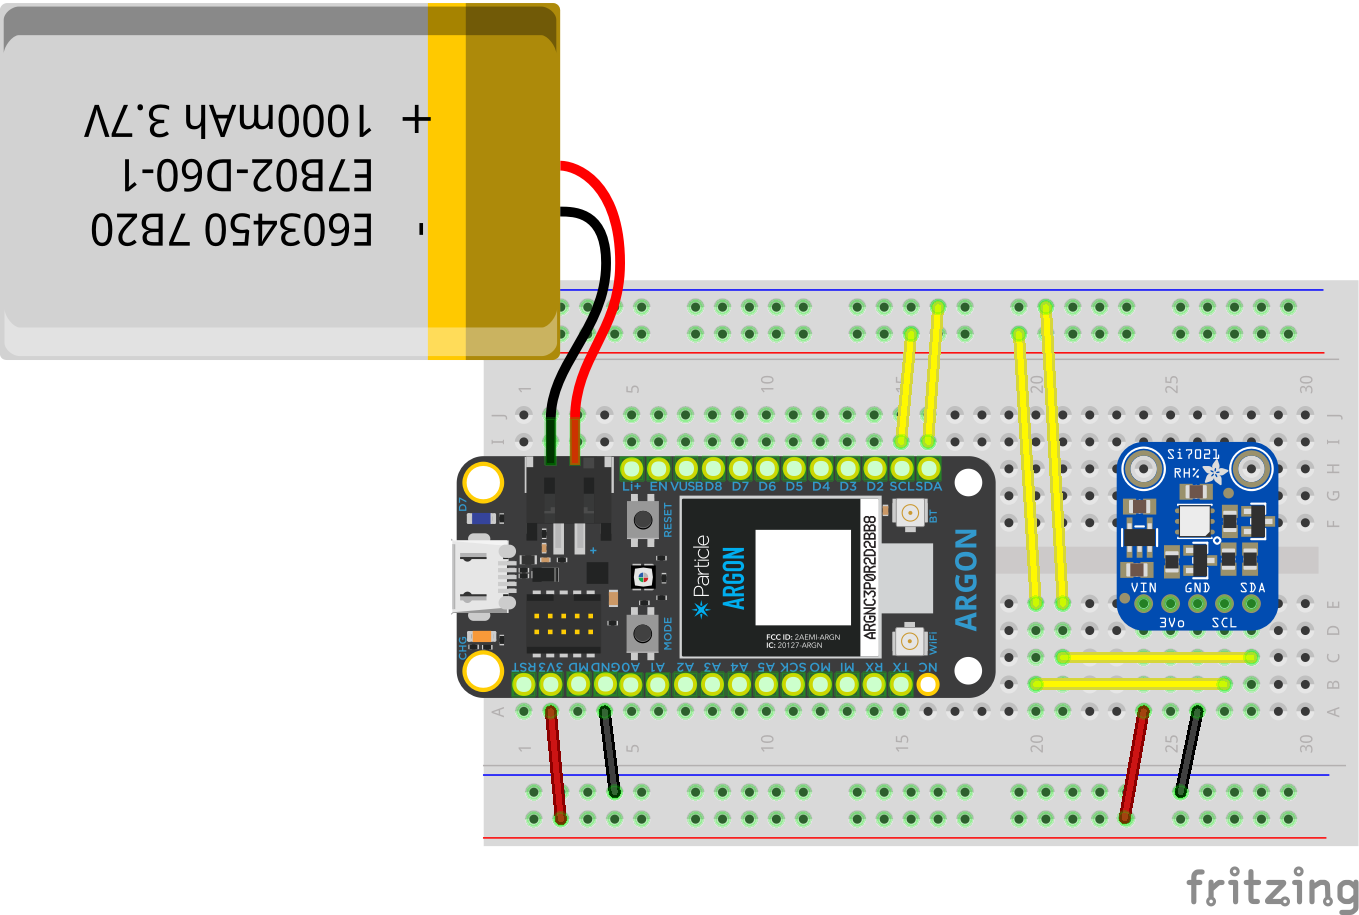
\includegraphics[width=\textwidth]{images/breadboard-schematic.png}
	\caption{Breadboard Schematic}
	\label{fig:breadboard_schematic}
\end{figure}

Figure~\ref{fig:breadboard_schematic} is the bread schematic showing how all of the hardware components are connected. This enables the Particle Argon to read and publish climate data events. With the battery, it makes the setup standalone and charged only when needed. Below is a brief description of each component.\\

\textbf{Particle Argon} — An IoT development kit for connecting to and sending information over the network.\\

\textbf{Adafruit Si7021} — A temperature and humidity sensor breakout board that provides the ability to read a given environment's climate.\\

\textbf{Breadboard} — A physical base that provides the ability to create circuits and prototype electronics.\\

\textbf{Jumper Wires} — Cables that can electrically connect components.\\

\textbf{Lithium Ion Polymer Battery 1000 mAh} — A power source for the connected components.

\subsection{Particle Argon and Particle Cloud}
\label{section:particle}
Particle Argon is flashed with firmware written with C code. It is used with Particle's API and the Adafruit Si7021 helper library. Understanding the Particle ecosystem's role in the system will reveal the scope of its interactions in the event-driven serverless architectural decision.

\begin{minipage}[c]{\textwidth}
	\begin{figure}[H]
		\lstinputlisting[language=C,firstline=9,lastline=12]{../src/particle-argon-temperature-humidity.ino}
		\caption{setup() function}
		\label{fig:setup}
	\end{figure}
\end{minipage}\ \\\\

The \textbf{setup()} as shown in Figure~\ref{fig:setup} is important here for two reasons. The first part is that the Particle Argon is in default timezone of Universal Time Coordinated (UTC) which differs from the timezone I live in is Central Daylight Time (CDT). To be able to represent the timezone difference, setting the default timezone with an offset of minus 5 hours is required. The second part is making sure that the Adafruit Si7021 is enabled after being initialized because it is the central piece for reading ambient temperature and relative humidity from a given environment.

\begin{minipage}[c]{\textwidth}
	\begin{figure}[H]
		\lstinputlisting[language=C,firstline=14,lastline=37]{../src/particle-argon-temperature-humidity.ino}
		\caption{loop() function}
		\label{fig:loop}
	\end{figure}
\end{minipage}\ \\\\

In Figure~\ref{fig:loop}, the \textbf{loop()} function shows that temperature and humidity are being read with the sensor object. They are then used as values to publish to the Particle Cloud. From that point on they are passed to Google Cloud Platform. However, there will be a further explanation of how this integration works and what processes happen on the Google Cloud Platform in Section~\ref{section:gcp}.

\begin{minipage}[c]{\textwidth}
	\begin{figure}[H]
		\lstinputlisting[language=C,firstline=39,lastline=55]{../src/particle-argon-temperature-humidity.ino}
		\caption{isEndOfDay() function}
		\label{fig:endofday}
	\end{figure}
\end{minipage}\ \\\\

Beyond publishing the climate values, the \textbf{loop()} function checks whether the day has ended from the perspective of the system. The end of the day is defined as code in Figure~\ref{fig:endofday}. Before it was mentioned that a UTC offset of minus 5 hours was applied in the \textbf{setup()} function, and this is where it comes into context. The end of the day is 9 PM CDT, which is equivalent to 21 in a 24-hour format. Once the system understands that it is the end of the day, an event is published to update a file containing daily climate average aggregates for the day. To understand the update itself will require digging into the Google Cloud Platform integration. As written before, this will be further explained in Section~\ref{section:functions}.\\

Concerning the end of the day as well as a variable called \textbf{publishIntervalMilliseconds} will be set to 1800000, in other words, 30 minutes. This publishing interval will last for 9 hours starting from 9 PM CDT to 6 AM CDT. During the working day, the \textbf{publishIntervalMilliseconds} is set to 900000, or 15 minutes. This plays a role in conserving battery because, during the night, it is only publishing climate data two per hour as opposed to four. However, the bigger battery-saving impact comes from placing the Particle Argon in a sleeping state.\\

A sleeping state means that the Particle Argon turns off all unnecessary internal processes that consume energy and maintains a low-power state for a duration of a configured time. There are two main modes of sleep state that Particle Argon can go into: \textbf{STOP} and \textbf{HIBERNATE}. The decision was to use the \textbf{STOP} sleeping mode because it provides the opportunity to keep the network connection alive while it is in a low-power state. \textbf{HIBERNATE} does not allow this, and if it was used, it would require the Particle Argon to completely establish a new connection every time it wakes up from the specified duration of \textbf{publishIntervalMilliseconds}; defeating the point of using it.

\subsection{Google Cloud Platform Services}
\label{section:gcp}
Google Cloud Platform is the most important part of the whole system. That being said, it is also important to give a brief description of each service used within the platform and why.

\subsubsection{Compute Engine}
\label{section:compute-engine}
Compute Engine is a virtual machine service that provides user-configured instances. This is as opposed to App Engine that is a fully-managed by Google Cloud Platform. The instance will be used to host a web server. With that, the system will have the ability to deliver a static website containing an interactive graph. Figure~\ref{fig:interactive-graph} shows ambient temperature and relative humidity daily averages that are data points on the interactive graph. The user will be able to see the changes over time and adjust the climate in their environment according to the purpose of what they are trying to achieve. It can be accessed in the link here: \url{http://35.238.110.48:8080}.

\begin{figure}[H]
	\center
	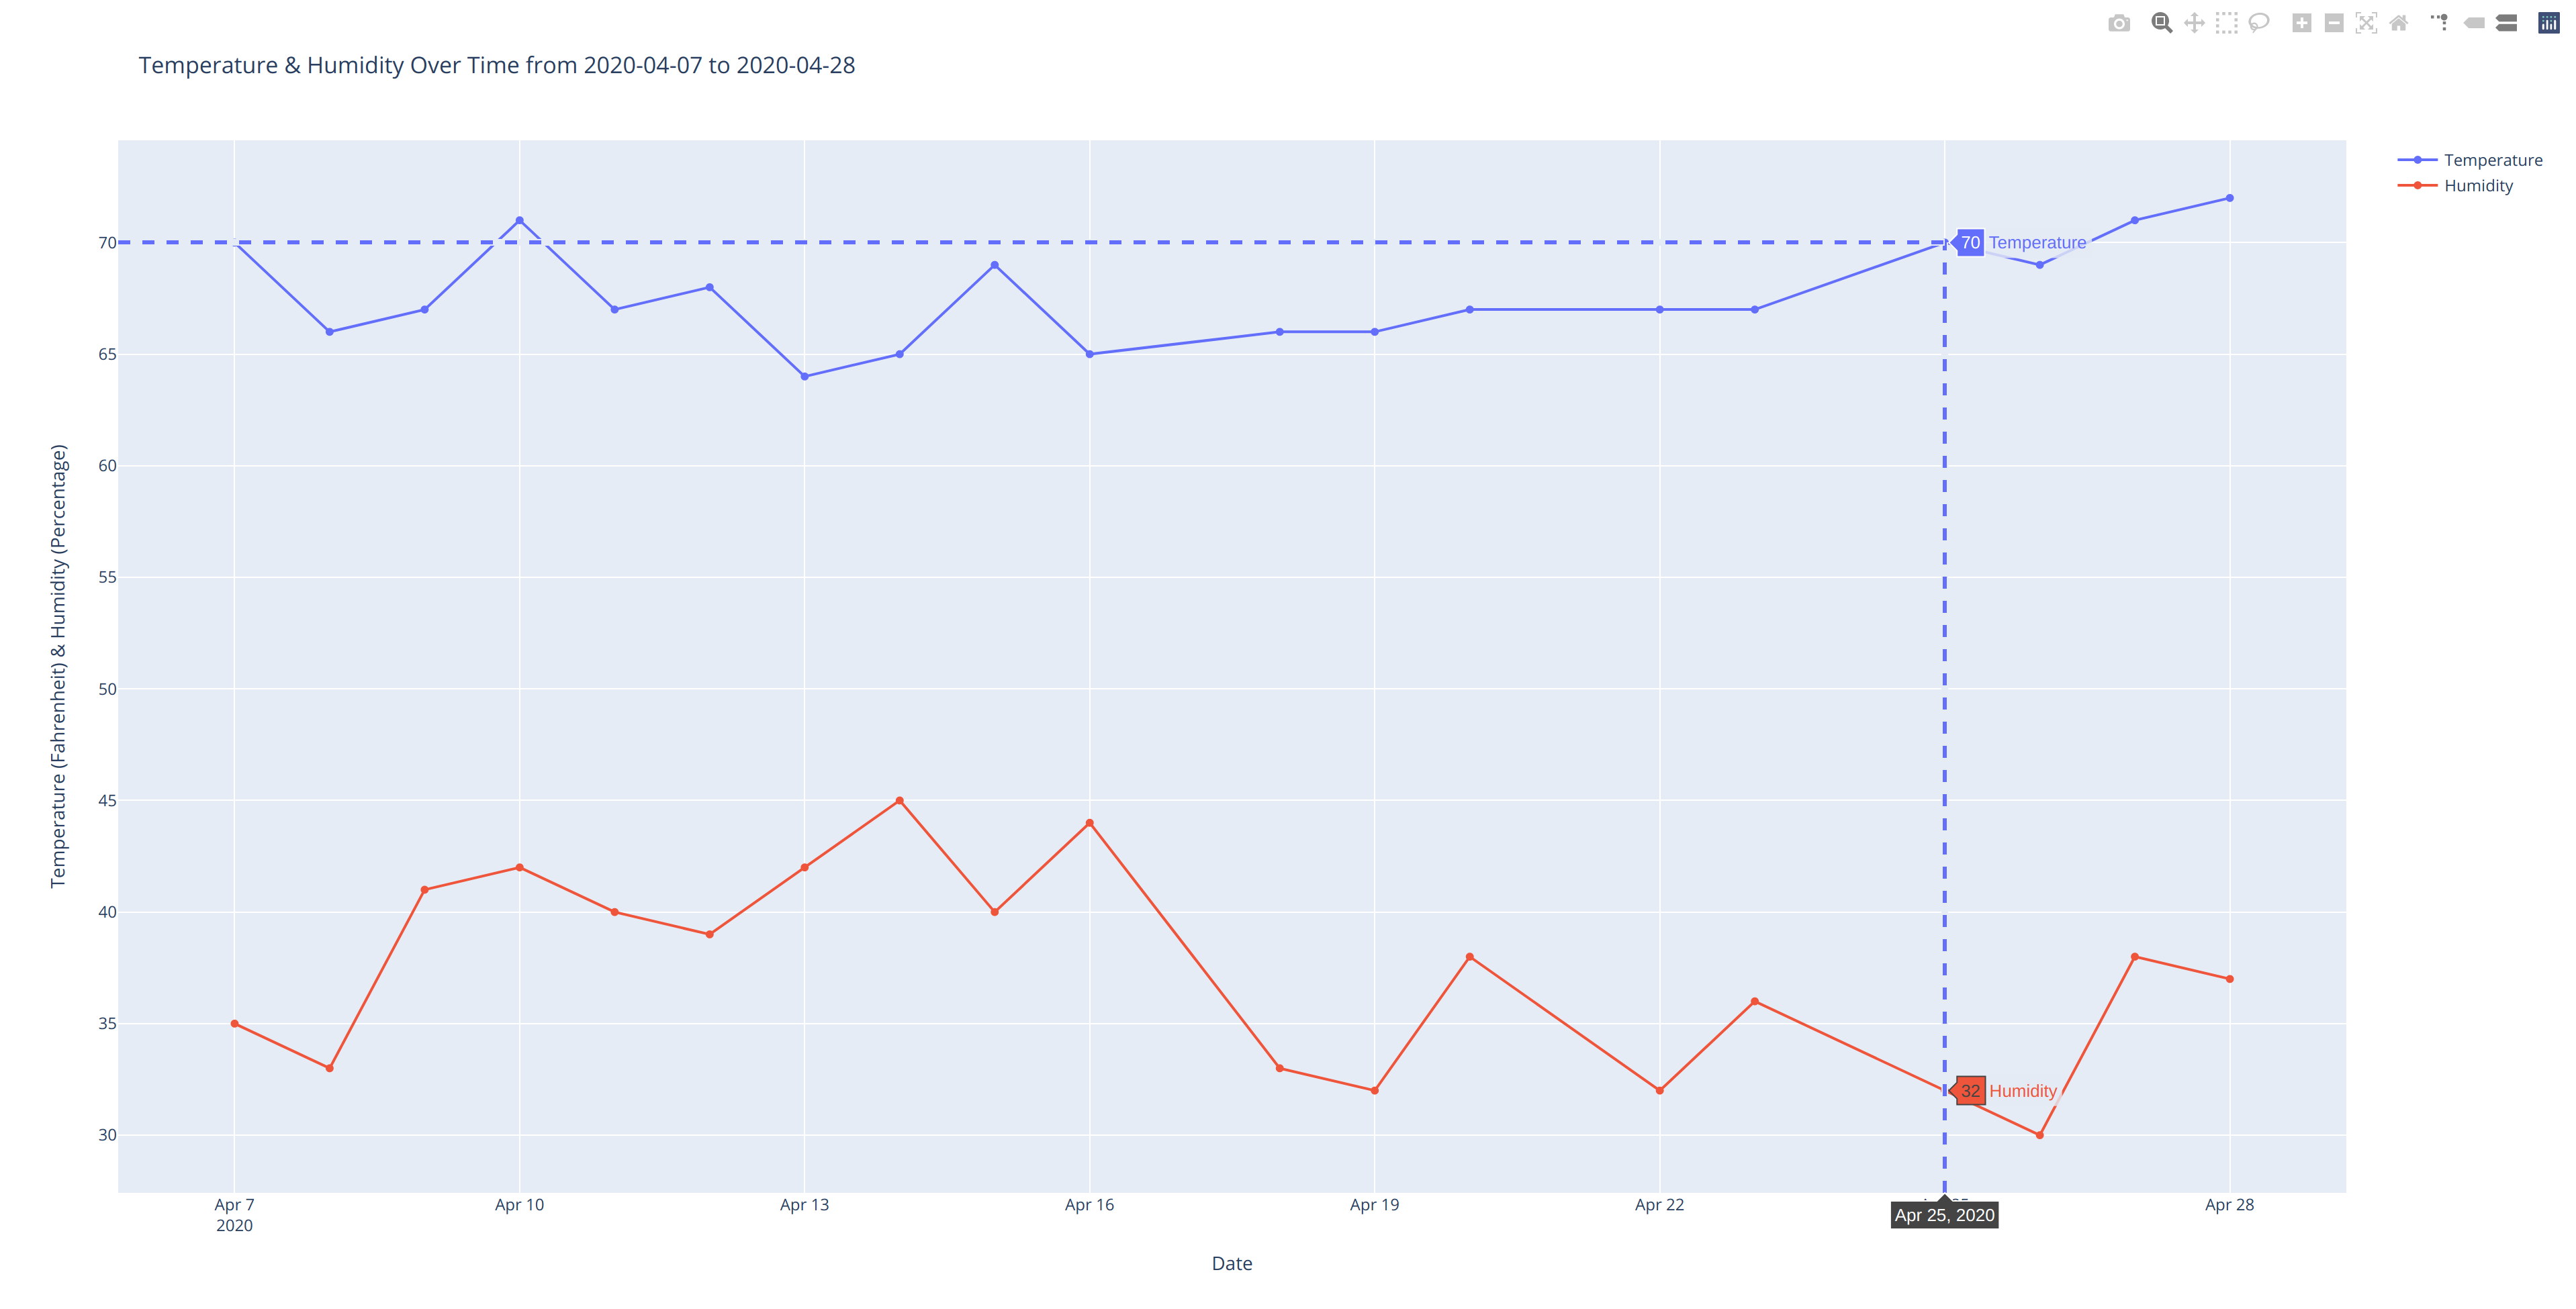
\includegraphics[width=\textwidth]{images/interactive-graph.png}
	\caption{Interactive Graph of Climate Data}
	\label{fig:interactive-graph}
\end{figure}

Previously it was mentioned that a web server was used to deliver the interactive graph, but the specifics of how that was accomplished were not explained. On a high level, it is a combination of using Python and several software components including Plotly, Docker, NGINX, and a separate project repository. Below will explain what each of these software components is and the role they play in the automatic creation and delivery of the graph to the web.\\

\textbf{Plotly} — A Python library to help develop custom graphs. It offers many graph types and visual options. To show climate data in a visually simple way, a line graph was used to indicate changing ambient temperature and relative humidity over time.\\

\textbf{Docker} — An OS-level containerization tool that can package software. Docker has a registry called Docker Hub full of container images created by the open-source community. These container images can be pulled down to a local machine and be used on-demand and/or developed on top of. These containers can be thought of as software building blocks to assist in software development.\\

\textbf{NGINX} — A web server that provides communication between client and server via HTTP. NGINX has container images stored in Docker Hub that is publicly accessible, which in this context, is used for standing up a web server in Compute Engine.\\

\textbf{Climate Data Graph Updater} — Updates the interactive graph on a daily basis when the \textbf{update\_climate\_data\_graph\_in\_engine()} trigger function is initiated, referenced in Section~\ref{section:functions}. This sits in a different GitHub repository from the Cloud Temperature \& Humidity Notification repository. The decision to isolate this portion of functionality was due to the lower operational cost of pulling it down from GitHub from the Compute Engine instance. It also separates the concern from the system perspective. The GitHub repository is linked here: \url{https://github.com/lxiong1/climate-data-graph-updater}.

\subsubsection{Firestore}
Firestore is a NoSQL document database that provides data persistence across the system. Specifically, this database is used for storing three major collections that assist in the state of the system. Figure~\ref{fig:contact-attempt-history},~\ref{fig:humidity}, and~\ref{fig:temperature} shows the different root collections and their respective documents.

\begin{figure}[H]
	\center
	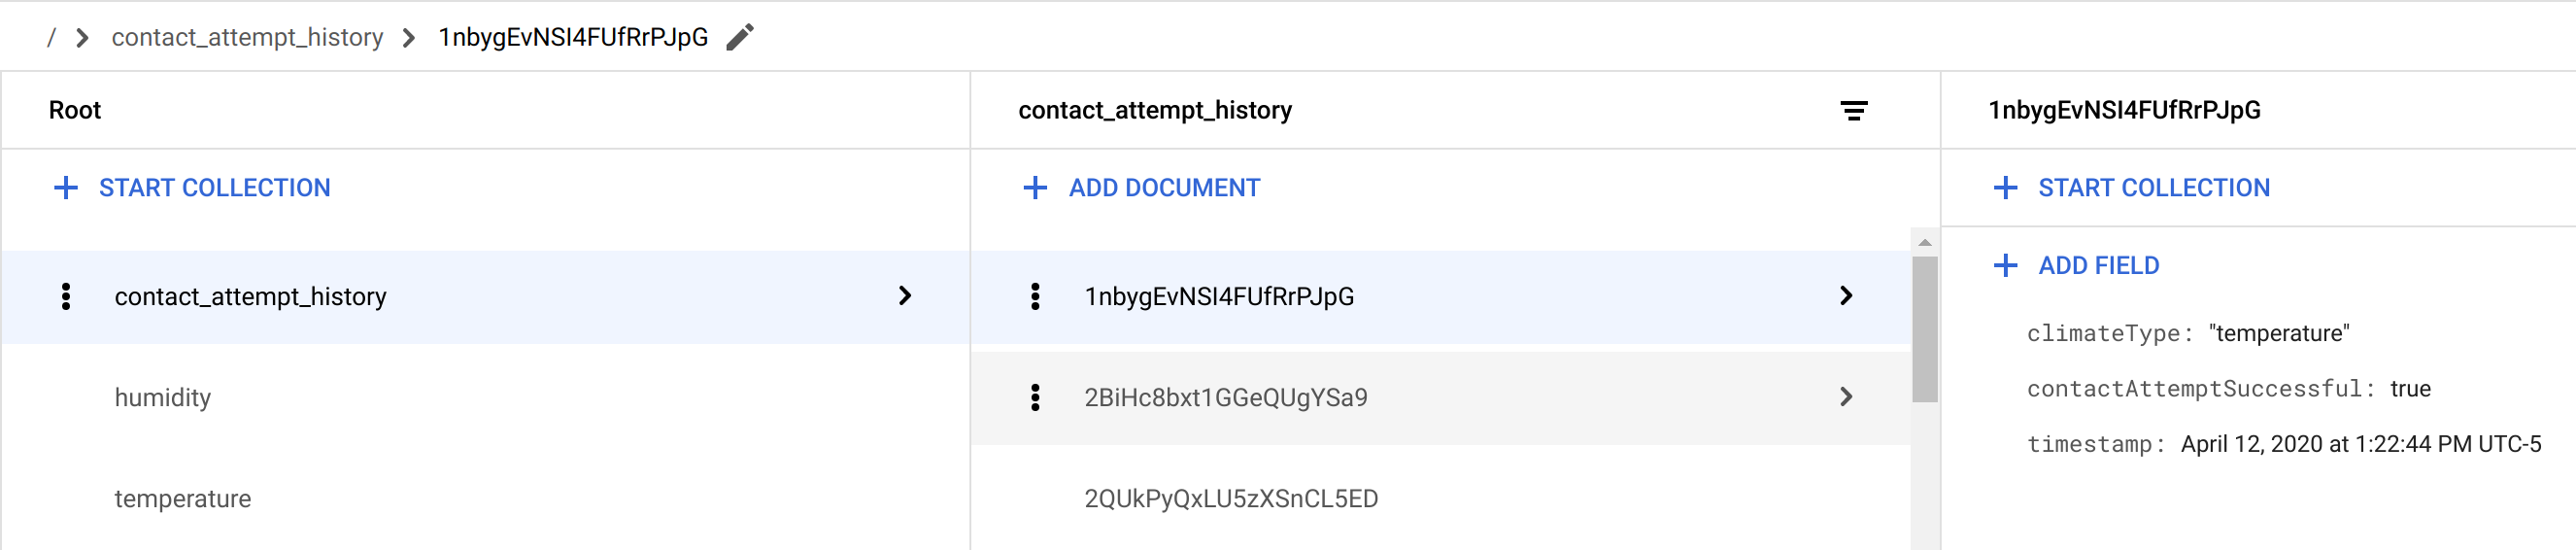
\includegraphics[width=\textwidth]{images/database-contact-attempt-history.png}
	\caption{Contact Attempt History Document}
	\label{fig:contact-attempt-history}
\end{figure}

\begin{figure}[H]
	\center
	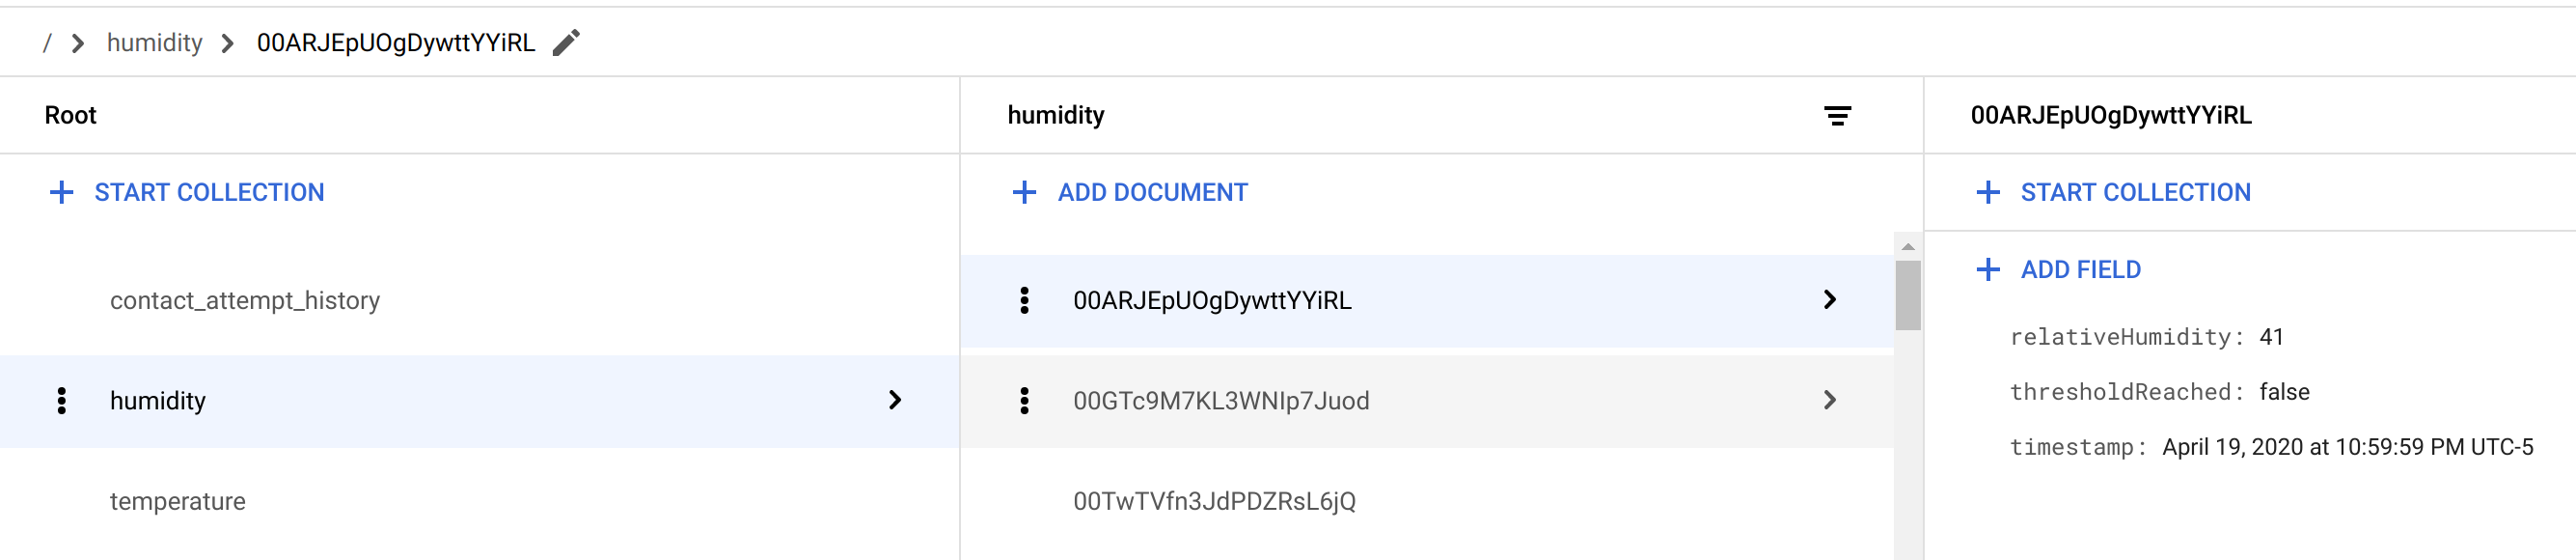
\includegraphics[width=\textwidth]{images/database-humidity.png}
	\caption{Relative Humidity Document}
	\label{fig:humidity}
\end{figure}

\begin{figure}[H]
	\center
	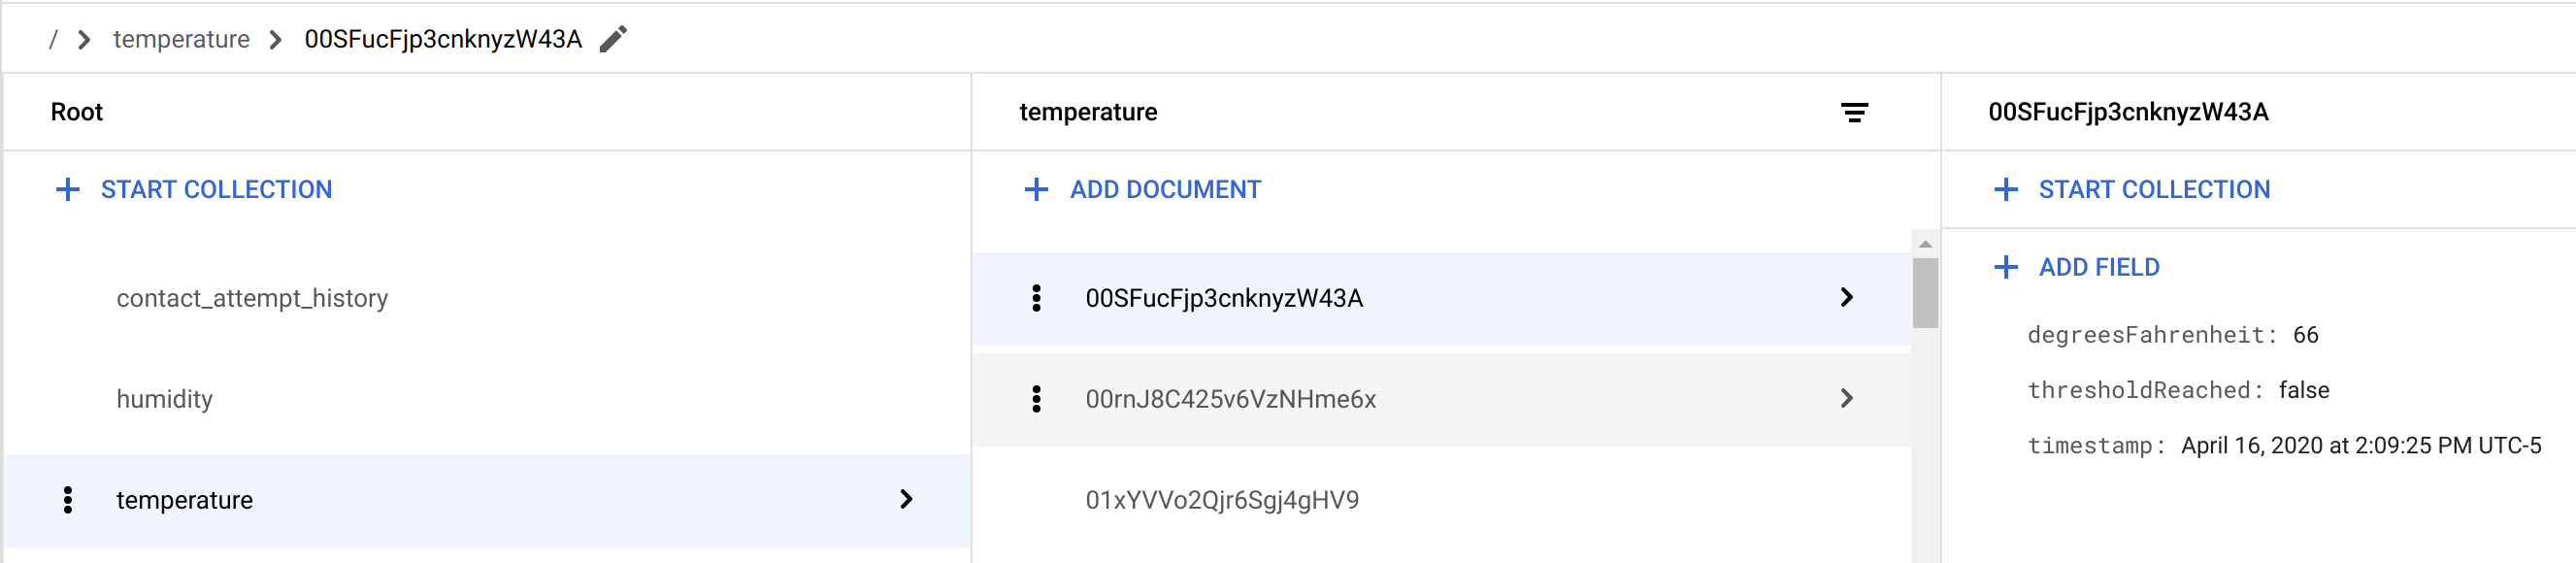
\includegraphics[width=\textwidth]{images/database-temperature.png}
	\caption{Ambient Temperture Document}
	\label{fig:temperature}
\end{figure}

As you can see, the root collections contain multiple documents with fields that contain data values. Each time a climate data or contact attempt event comes through the system, a new document is created for each of those events to ensure that the system understands what historically has occurred.

\subsubsection{Functions}
\label{section:functions}
Functions is an event-driven serverless compute service. This is the heart and soul of the Cloud Temperature \& Humidity Notification System. This is where most of the computation happens. As outlined in Section~\ref{section:architecture}, there are major advantages of using a service like Functions that align with being event-driven serverless. Figure~\ref{fig:functions} shows the existing serverless functions of the system.\\

\begin{figure}[H]
	\center
	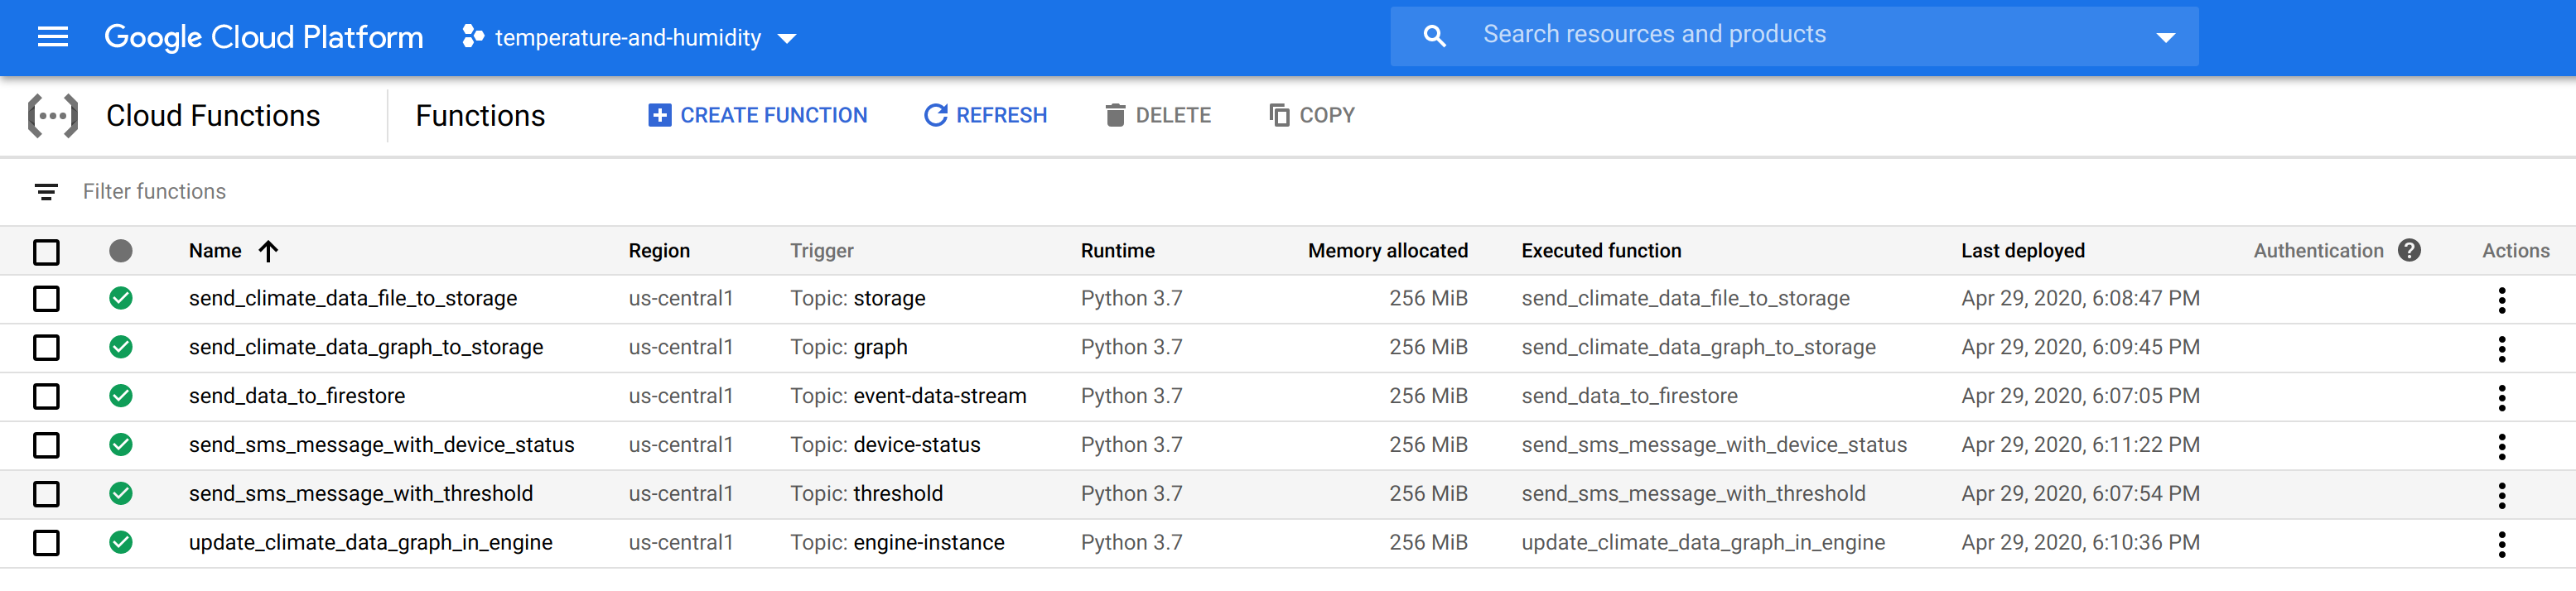
\includegraphics[width=\textwidth]{images/serverless-functions.png}
	\caption{Google Cloud Functions}
	\label{fig:functions}
\end{figure}

A convenient feature about Functions is that it allows engineers to test all code written to be tested from anywhere. An engineer can deploy a serverless function to be deployed and then tested in a controlled environment or from a local machine. There simply is no limitation to where these serverless functions run. From first-hand experience, being able to test locally helps reduce unnecessary deploy time, which can take up to a couple of minutes and even up to a minute afterward to properly register.\\

It's important to point out that Section~\ref{section:pubsub} and this section are tightly related. Refer to Figure~\ref{fig:mapping} to see the association of trigger functions to their respective PubSub topics. Topics will relay events (AKA messages) to these trigger functions to perform some action. What this action encompasses depends on the event.\\

\begin{figure}[H]
	\center
	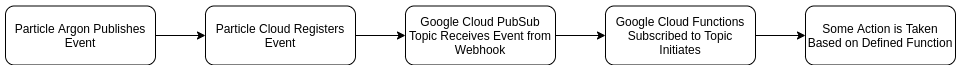
\includegraphics[width=\textwidth]{images/generic-temperature-humidity-flow.png}
	\caption{Generic System Event Flow}
	\label{fig:event-flow}
\end{figure}

Figure ~\ref{fig:event-flow} shows the general event flow starting from the Particle Argon to the serverless function. The specifics of what happens after an event type makes this process more complex. To better understand the specifics of the system, take a look at Figure~\ref{fig:climate-event-flow}. Though it is specifically referring to temperature events, humidity events have the same flow throughout the system.

\begin{figure}[H]
	\center
	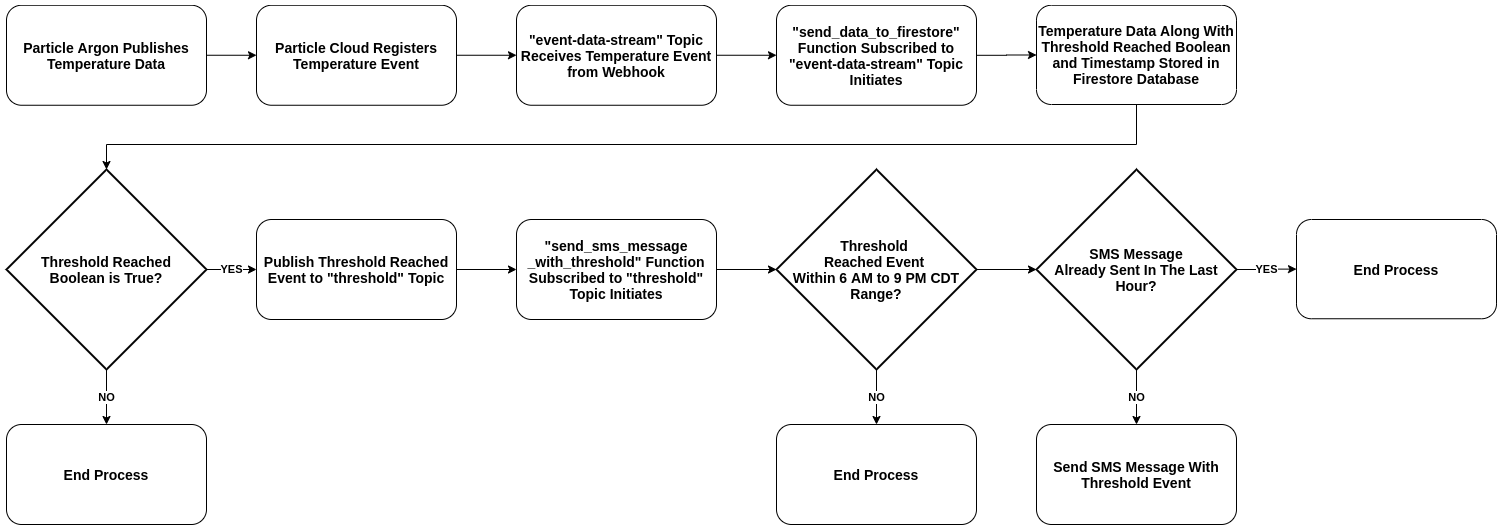
\includegraphics[width=\textwidth]{images/climate-event-flow.png}
	\caption{Temperature Event Flow Within System}
	\label{fig:climate-event-flow}
\end{figure}

Figure~\ref{fig:climate-event-flow} demonstrates how an SMS message is determined to be sent to a user. In the event flow, there is what is called \textbf{Trigger Function Chaining}. A function can send a message to another topic which then initiates a different function, thus why it is referred to as chaining. The functions themselves hold absolutely no state of the system, it searches in the database to understand the state. Notice how the \textbf{Threshold Reached} boolean value was stored into the database to determine whether there should be a potential SMS message to be sent out. That is the database storing the state, not the function itself. This separation of concern is crucial to properly build out an event-driven serverless system.

\begin{figure}[H]
	\center
	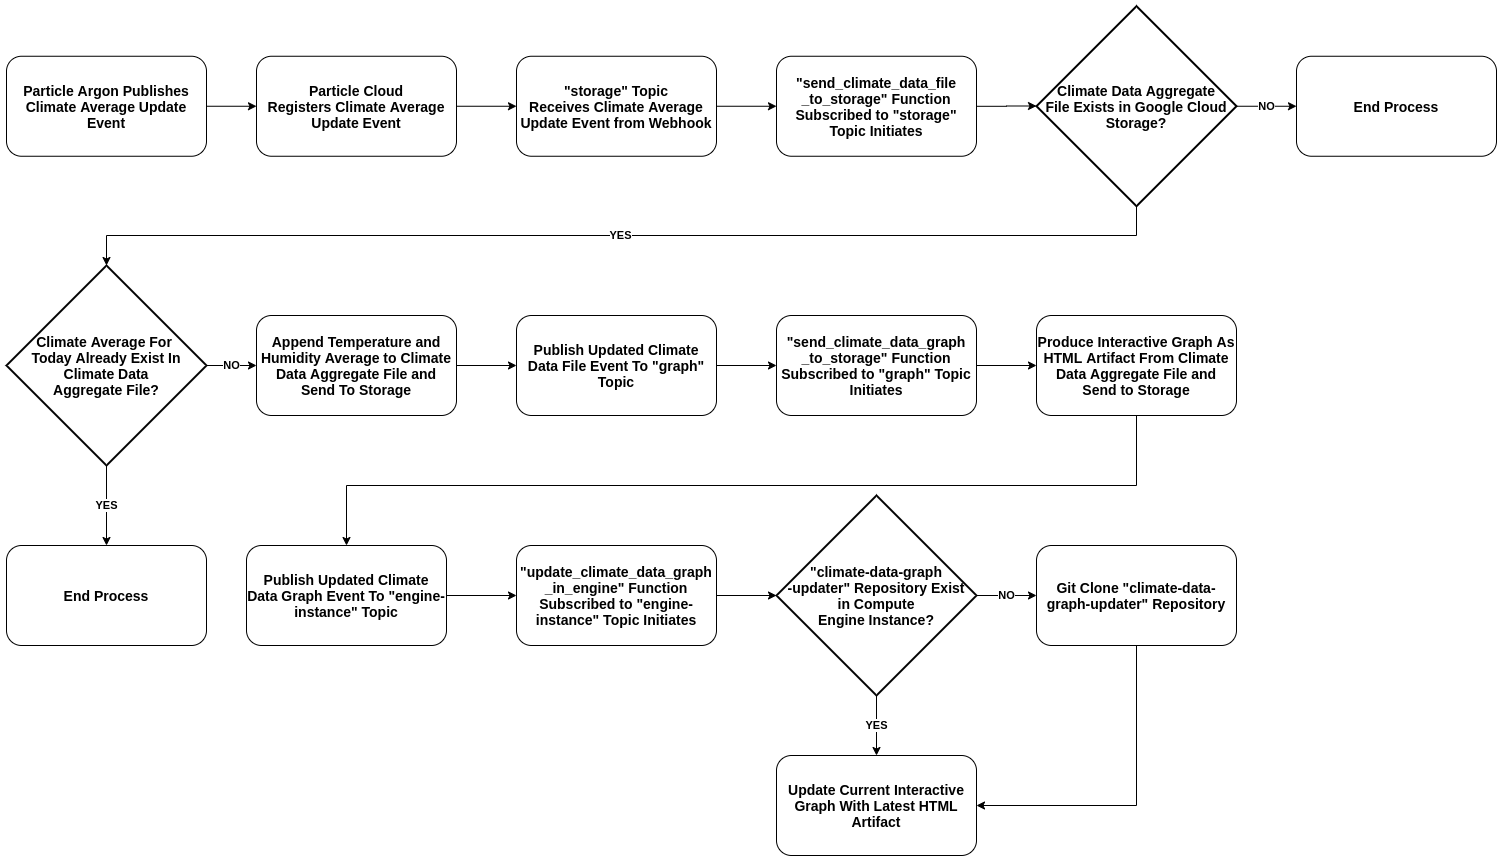
\includegraphics[width=\textwidth]{images/graph-event-flow.png}
	\caption{Climate Average Update Event Flow Within System}
	\label{fig:graph-event-flow}
\end{figure}

To update the interactive graph \url{http://35.238.110.48:8080}, Figure ~\ref{fig:graph-event-flow} demonstrates the processing that has to occur. It was mentioned before in Section~\ref{section:particle} that the prerequisite for this update to begin, is when it is the end of the day, namely, 9 PM CDT. This process uses Trigger Function Chaining just as does when a temperature or humidity event is sent. The last functionality of the system is checking for the device status of the Particle Argon.

\begin{figure}[H]
	\center
	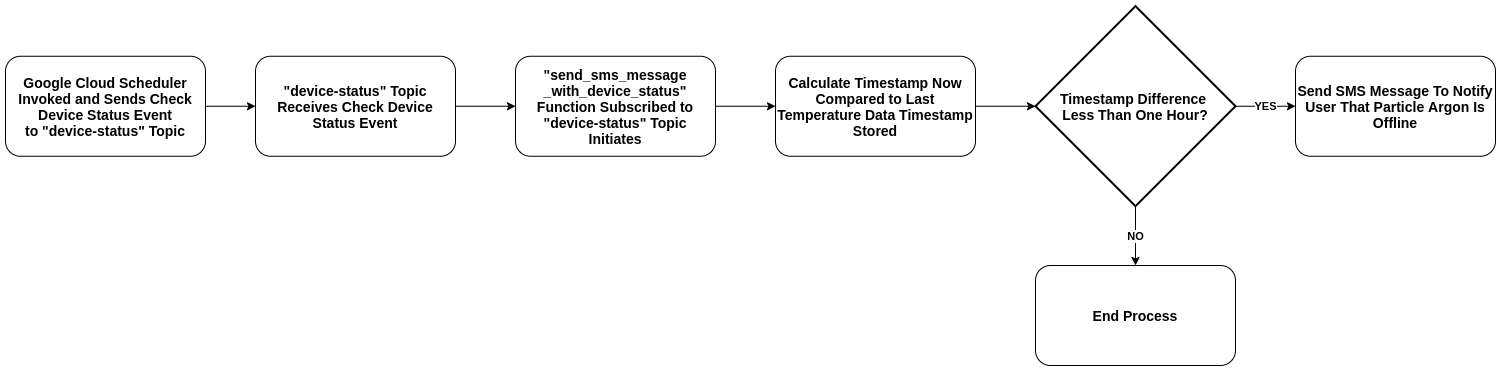
\includegraphics[width=\textwidth]{images/device-status-event-flow.png}
	\caption{Device Status Event Flow Within System}
	\label{fig:device-status-event-flow}
\end{figure}

This is where the Google Cloud Scheduler explained in Section~\ref{section:scheduler} is used. Every hour of the working day -- defined as 6 AM to 9 PM CDT, the Scheduler will send a message to the "device-status" topic and check whether the Particle Argon is offline or online. Figure~\ref{fig:device-status-event-flow} goes into detail of what that event flow looks like.\\

As a late note on this section, code was not specifically covered in here due to the large amount of code. Also it was not necessary as the diagrams explain what the serverless functions code does. However all Python code written for the serverless functions can be found here:\\

\url{https://github.com/lxiong1/cloud-temperature-humidity-notification/tree/master/functions}

\subsubsection{PubSub}
\label{section:pubsub}
PubSub is an asynchronous middleware messaging service. The base for this service revolves around three major concepts of topics, subscriptions, and messages. Topics are where messages are sent to when published. Subscriptions are the message retrievers when a message is published to the topic they are associated with. Messages are are the data published to topics and streamed to subscribers.

\begin{figure}[H]
	\center
	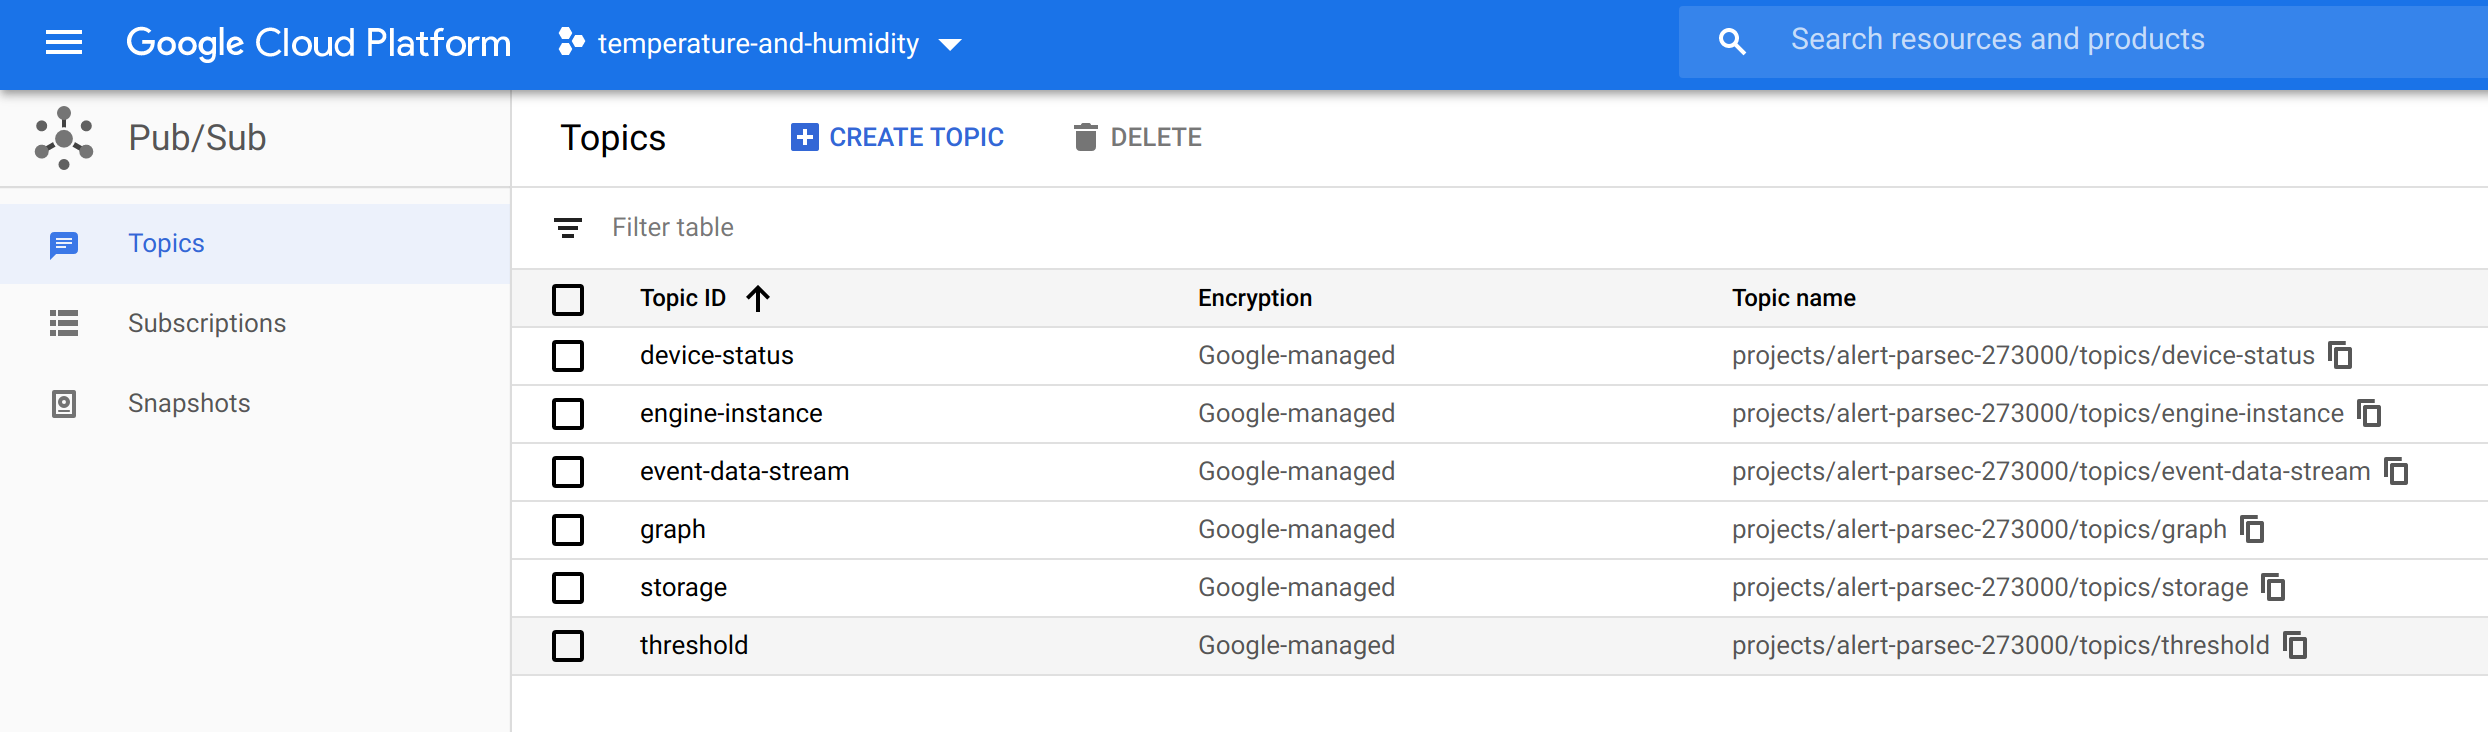
\includegraphics[width=\textwidth]{images/pubsub-topics.png}
	\caption{Google Cloud PubSub Topics}
	\label{fig:pubsub-topics}
\end{figure}

The advantage of using PubSub is that messages can be sent from anywhere and at any scale. There is no need to manage to scale as PubSub enacts the scaling needs automatically. This is a part of what makes the system event-driven serverless. It consumes messages and passes the information along as directed without standing up and configuring any server. It just works.\\

In the system context, messages are the events published by Particle Argon. Figure~\ref{fig:pubsub-topics} shows all of the existing topics that support events processing. These topics are the first point of contact with the Particle ecosystem, starting from the Particle Argon publishing its events to the Particle Cloud and those events being webhooked into the PubSub topics. Every time an event is published to a topic, a subscribed trigger function initiates. Figure~\ref{fig:mapping} is a mapping of topics and their subscribed trigger functions.\\

\begin{figure}[H]
	\begin{lstlisting}
    TRIGGER_FUNCTION_NAME: send_data_to_firestore
    TOPIC_NAME: event-data-stream

    TRIGGER_FUNCTION_NAME: send_sms_message_with_threshold
    TOPIC_NAME: threshold

    TRIGGER_FUNCTION_NAME: send_climate_data_file_to_storage
    TOPIC_NAME: storage

    TRIGGER_FUNCTION_NAME: send_climate_data_graph_to_storage
    TOPIC_NAME: graph

    TRIGGER_FUNCTION_NAME: update_climate_data_graph_in_engine
    TOPIC_NAME: engine-instance

    TRIGGER_FUNCTION_NAME: send_sms_message_with_device_status
    TOPIC_NAME: device-status
    \end{lstlisting}
	\caption{Mapping of Subscribed Trigger Functions to PubSub Topics}
	\label{fig:mapping}
\end{figure}

\subsubsection{Scheduler}
\label{section:scheduler}
Scheduler is Cron job scheduler fully-managed by Google Cloud Platform. It would be wise to explain what Cron because it is not common knowledge. To put it simply, Cron is a Unix utility for scheduling arbitrary processes to run at arbitrary times. For example, Figure~\ref{fig:scheduler} shows that the system defines \textbf{0 6-21 * * * (America/Chicago)} under the frequency column. This is UNIX-Cron format for time-based scheduling and translates to, "every day every hour from 6 AM to 9 PM CDT."

\begin{figure}[H]
	\center
	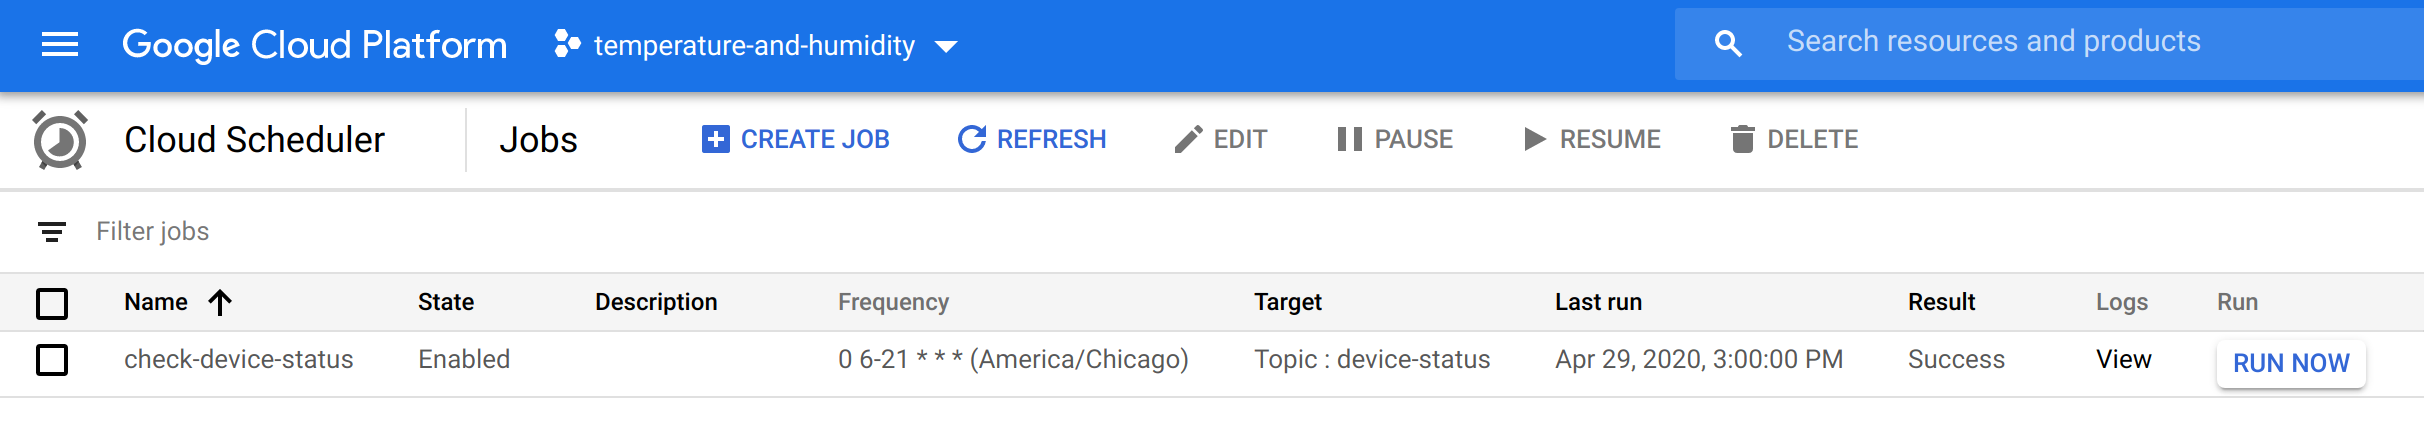
\includegraphics[width=\textwidth]{images/scheduler.png}
	\caption{Google Cloud Scheduler}
	\label{fig:scheduler}
\end{figure}

What exact process is running for the system? As the name \textbf{check-device-status} from Figure~\ref{fig:scheduler} suggests, it sends an event to a PubSub topic called \textbf{device-status} that ultimately checks whether the device status is online or offline. For more information on the details of how that works, refer to Section~\ref{section:functions}.

\subsubsection{Identity and Access Management}
Identity and Access Management (IAM) is a service that provides the ability to manage roles and permissions on Google Cloud Platform resources. This is extremely important to manage correctly as giving people more access than they need can potentially compromise a system entirely. Google Cloud Platform takes the approach of a zero-trust security model, so existing resources have to be given appropriate roles and permissions by the administrator.

\subsubsection{Secret Manager}
Secret Manager provides security around creating, storing, accessing, versioning, and destroying secrets. Many companies struggle with managing their secrets and often overlook the need for security for the sake of convenience. Although Secret Manager makes it easier to do this, it can be incredibly complex depending on the security needs of an organization.

\begin{figure}[H]
	\center
	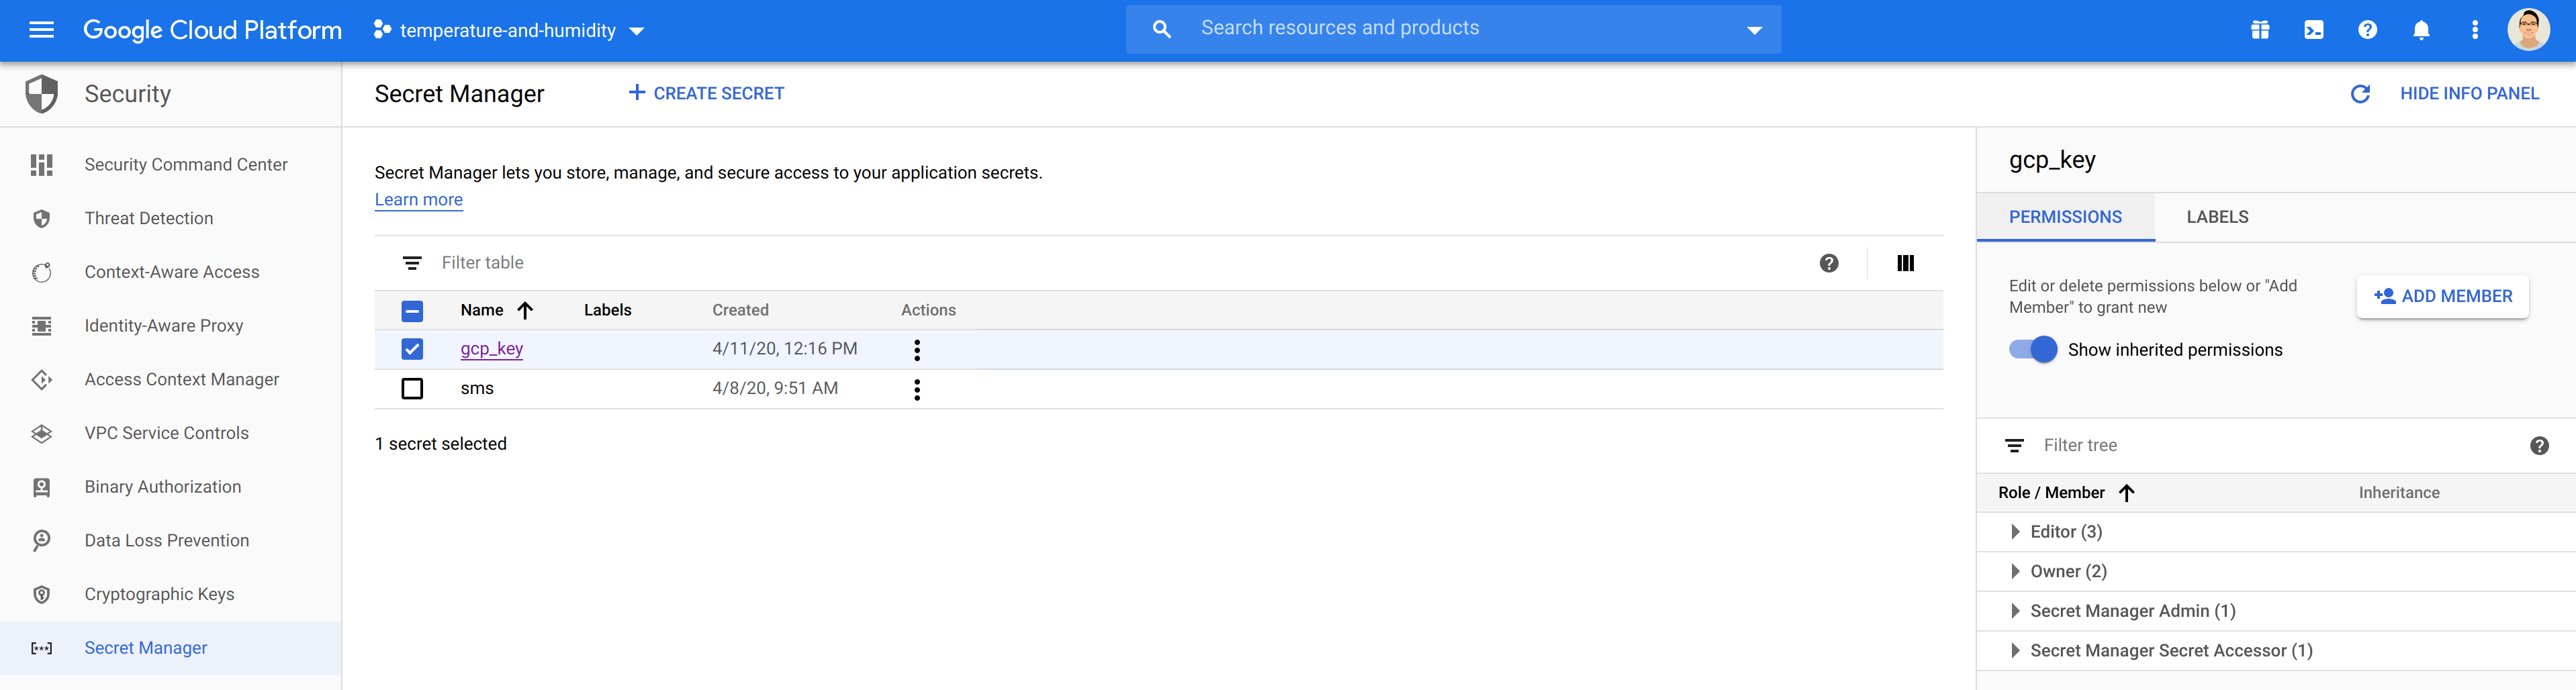
\includegraphics[width=\textwidth]{images/secret-manager.png}
	\caption{Google Cloud Secret Manager}
	\label{fig:secret-manager}
\end{figure}

There are currently two secrets stored as shown in Figure~\ref{fig:secret-manager}. They are automatically retrieved for usage when certain events come through the system. The \textbf{gcp\_key} secret is used to Secure Shell (SSH) into the Compute Engine instance to update the interactive graph from a trigger function, explained in Section~\ref{section:functions}. The \textbf{sms} secret is used for authenticating to an email account used solely to send out SMS messages, also explained the Section~\ref{section:functions}.

\subsubsection{Storage}
Storage is a web file storage service. To store files in the service, users have to create what Google Cloud Platform calls a \textbf{Bucket}. A Bucket is just a way to categorize content, comparable to the way a Linux filesystem is structured with directory and files. For the system, one bucket was created and called \textbf{climate-data-files}. In it contains two files that are foundational to auto-updating the interactive graph referenced in Section~\ref{section:compute-engine}.

\begin{figure}[H]
	\center
	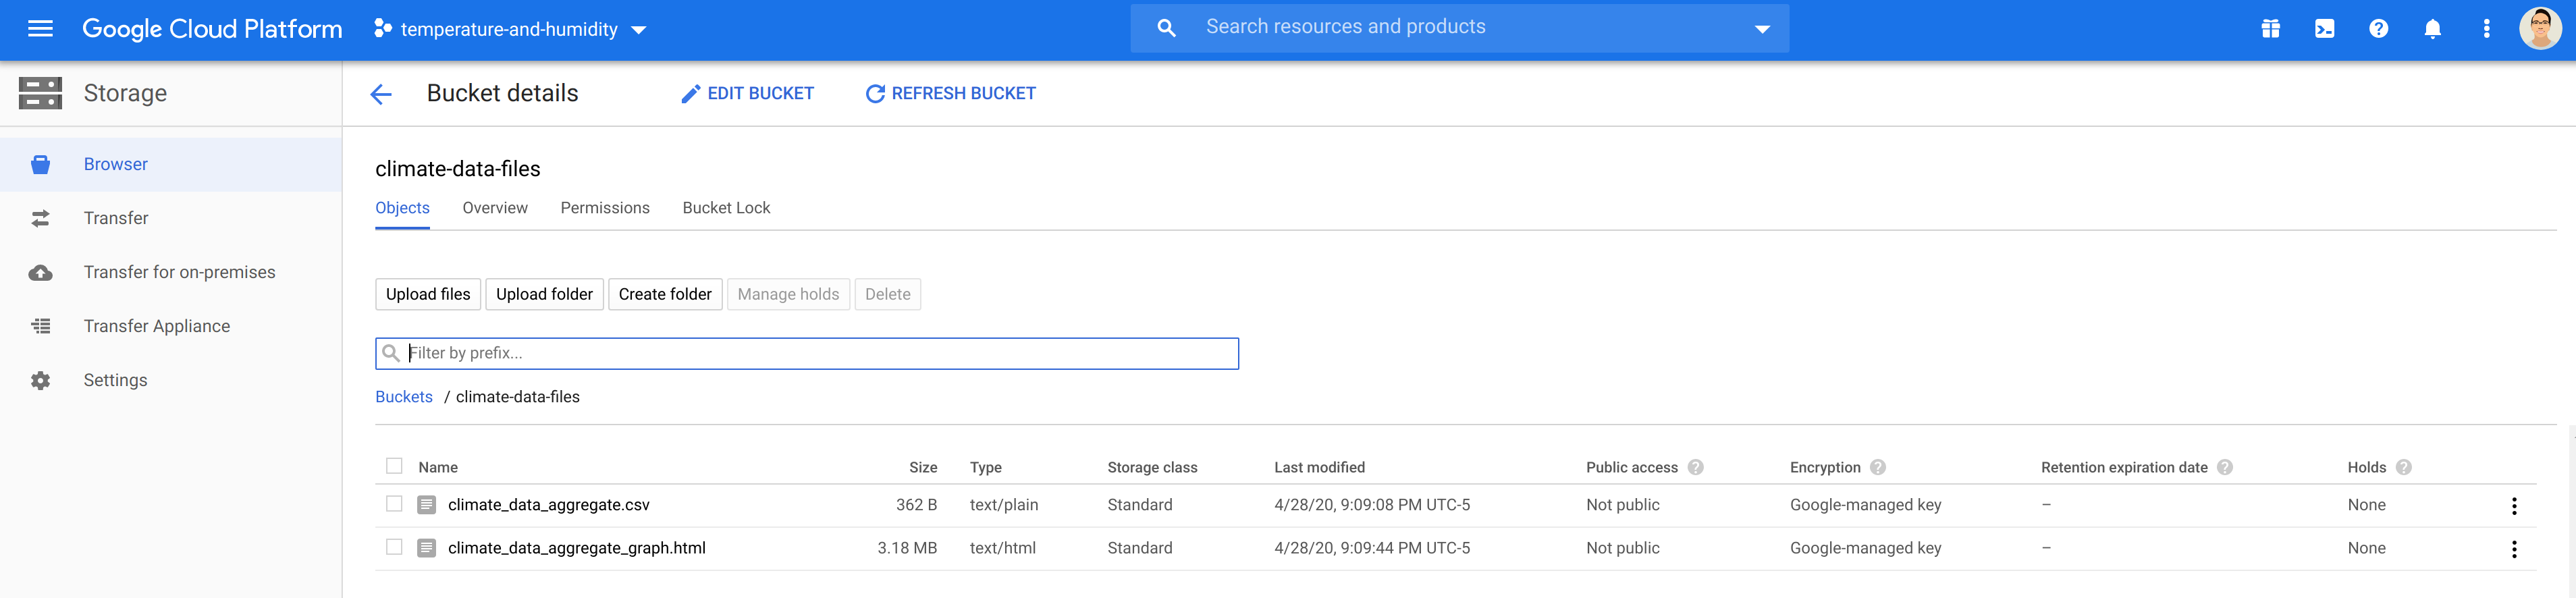
\includegraphics[width=\textwidth]{images/storage.png}
	\caption{Google Cloud Storage}
	\label{fig:storage}
\end{figure}

The first file is called \textbf{climate\_data\_aggregate.csv} and its contents are comma-delimited average temperature and humidity data values as well as the date. Refer to Figure~\ref{fig:climate-data} for a visual. It is the base for updating the second file called \textbf{climate\_data\_aggregate\_graph.html}. The HTML file ultimately ends up being used for updating the interactive graph.

\begin{figure}[H]
	\center
	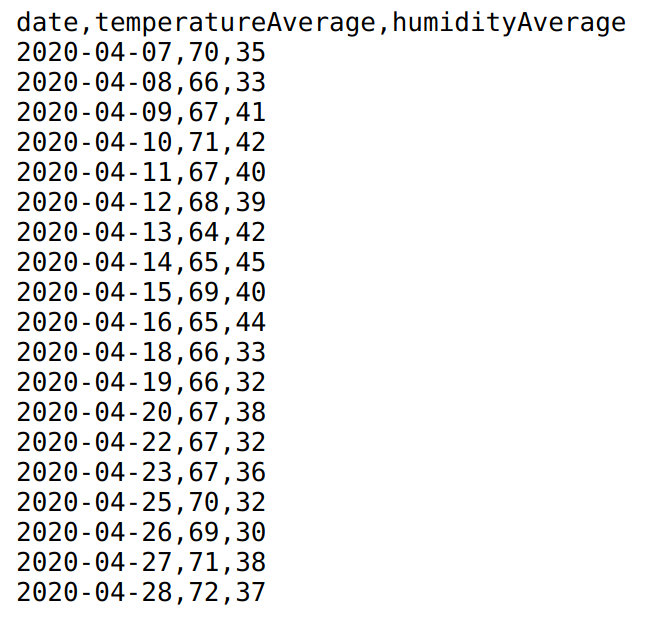
\includegraphics[width=.6\textwidth]{images/climate-data-csv.png}
	\caption{Average Climate Data from Aggregate CSV file}
	\label{fig:climate-data}
\end{figure}

\subsection{GitHub Actions}
With all of the development effort that has gone into building out the system, there was a need to simplify the deployment process. This process usually involved manually typing long commands in the terminal repetitively as the system iterations happened. The rule of thumb for software engineers is this: if you have to do it more than once, just automate it. This is where GitHub Actions comes into play.\\

Self-explanatory in its name of who the creator is, GitHub Actions is a platform created to automate workflows. In essence, it is a Continuous Integration (CI) and Continuous Delivery/Deployment (CD) tool for software engineers that want to simplify and reduce repetitive tasks. GitHub Actions has helped remove the repetitive tasks that involve deploying the source code into production.

\begin{figure}[H]
	\begin{figure}[H]
		\lstinputlisting[firstline=1,lastline=9]{../.github/workflows/master-workflow.yml}
		\caption{Part-one master-workflow.yml}
		\label{fig:workflow-file-one}
	\end{figure}
\end{figure}

Figure~\ref{fig:workflow-file-one} shows the \textbf{master-workflow.yml} containing the instructions to run on a push to the Master branch and only when functions directory's contents have been changed. Otherwise, the automated pipeline does not run. The reason for this is because the serverless functions are the only concern in terms of deployment.

\begin{figure}[H]
	\begin{figure}[H]
		\lstinputlisting[firstline=10,lastline=35]{../.github/workflows/master-workflow.yml}
		\caption{Part-two master-workflow.yml}
		\label{fig:workflow-file-two}
	\end{figure}
\end{figure}

Figure~\ref{fig:workflow-file-two} shows the setup portion of the workflow that runs after the workflow trigger criteria is met as a result of the workflow defined in Figure~\ref{fig:workflow-file-one}. This will check out the source code, setup Python and run the Python code formatter as well as the code linter, and then finish up by gaining API access to Google Cloud Platform. The secrets that are needed to gain this access is stored within GitHub, and will only be retrieved at runtime for security purposes. At any point that any of these steps fail, it will stop the whole pipeline and throw an error.\\

The actual deployment is shown in Figure~\ref{fig:workflow-file-three} is the key reason for the automated pipeline. Each of the serverless functions that exist within the functions directory will be deployed and associated with each of their respective Google PubSub topics. This portion takes the longest but since it is automated, it makes deployment much faster and easier. In summary, no more manual setup and deployments in the terminal.

\begin{figure}[H]
	\begin{figure}[H]
		\lstinputlisting[firstline=36,lastline=65]{../.github/workflows/master-workflow.yml}
		\caption{Part-three master-workflow.yml}
		\label{fig:workflow-file-three}
	\end{figure}
\end{figure}

It is crucial to point out the inherent benefit of building an automated workflow on such a platform, that is, idempotency. Machines only run the instructions they have been given and nothing more. It means that an engineer can expect the same results whenever their pipeline runs. Figure~\ref{fig:workflow-visual} is a visual for engineers to see the automated pipeline step by step that ran after a push to the Master branch.\\

\begin{figure}[H]
	\center
	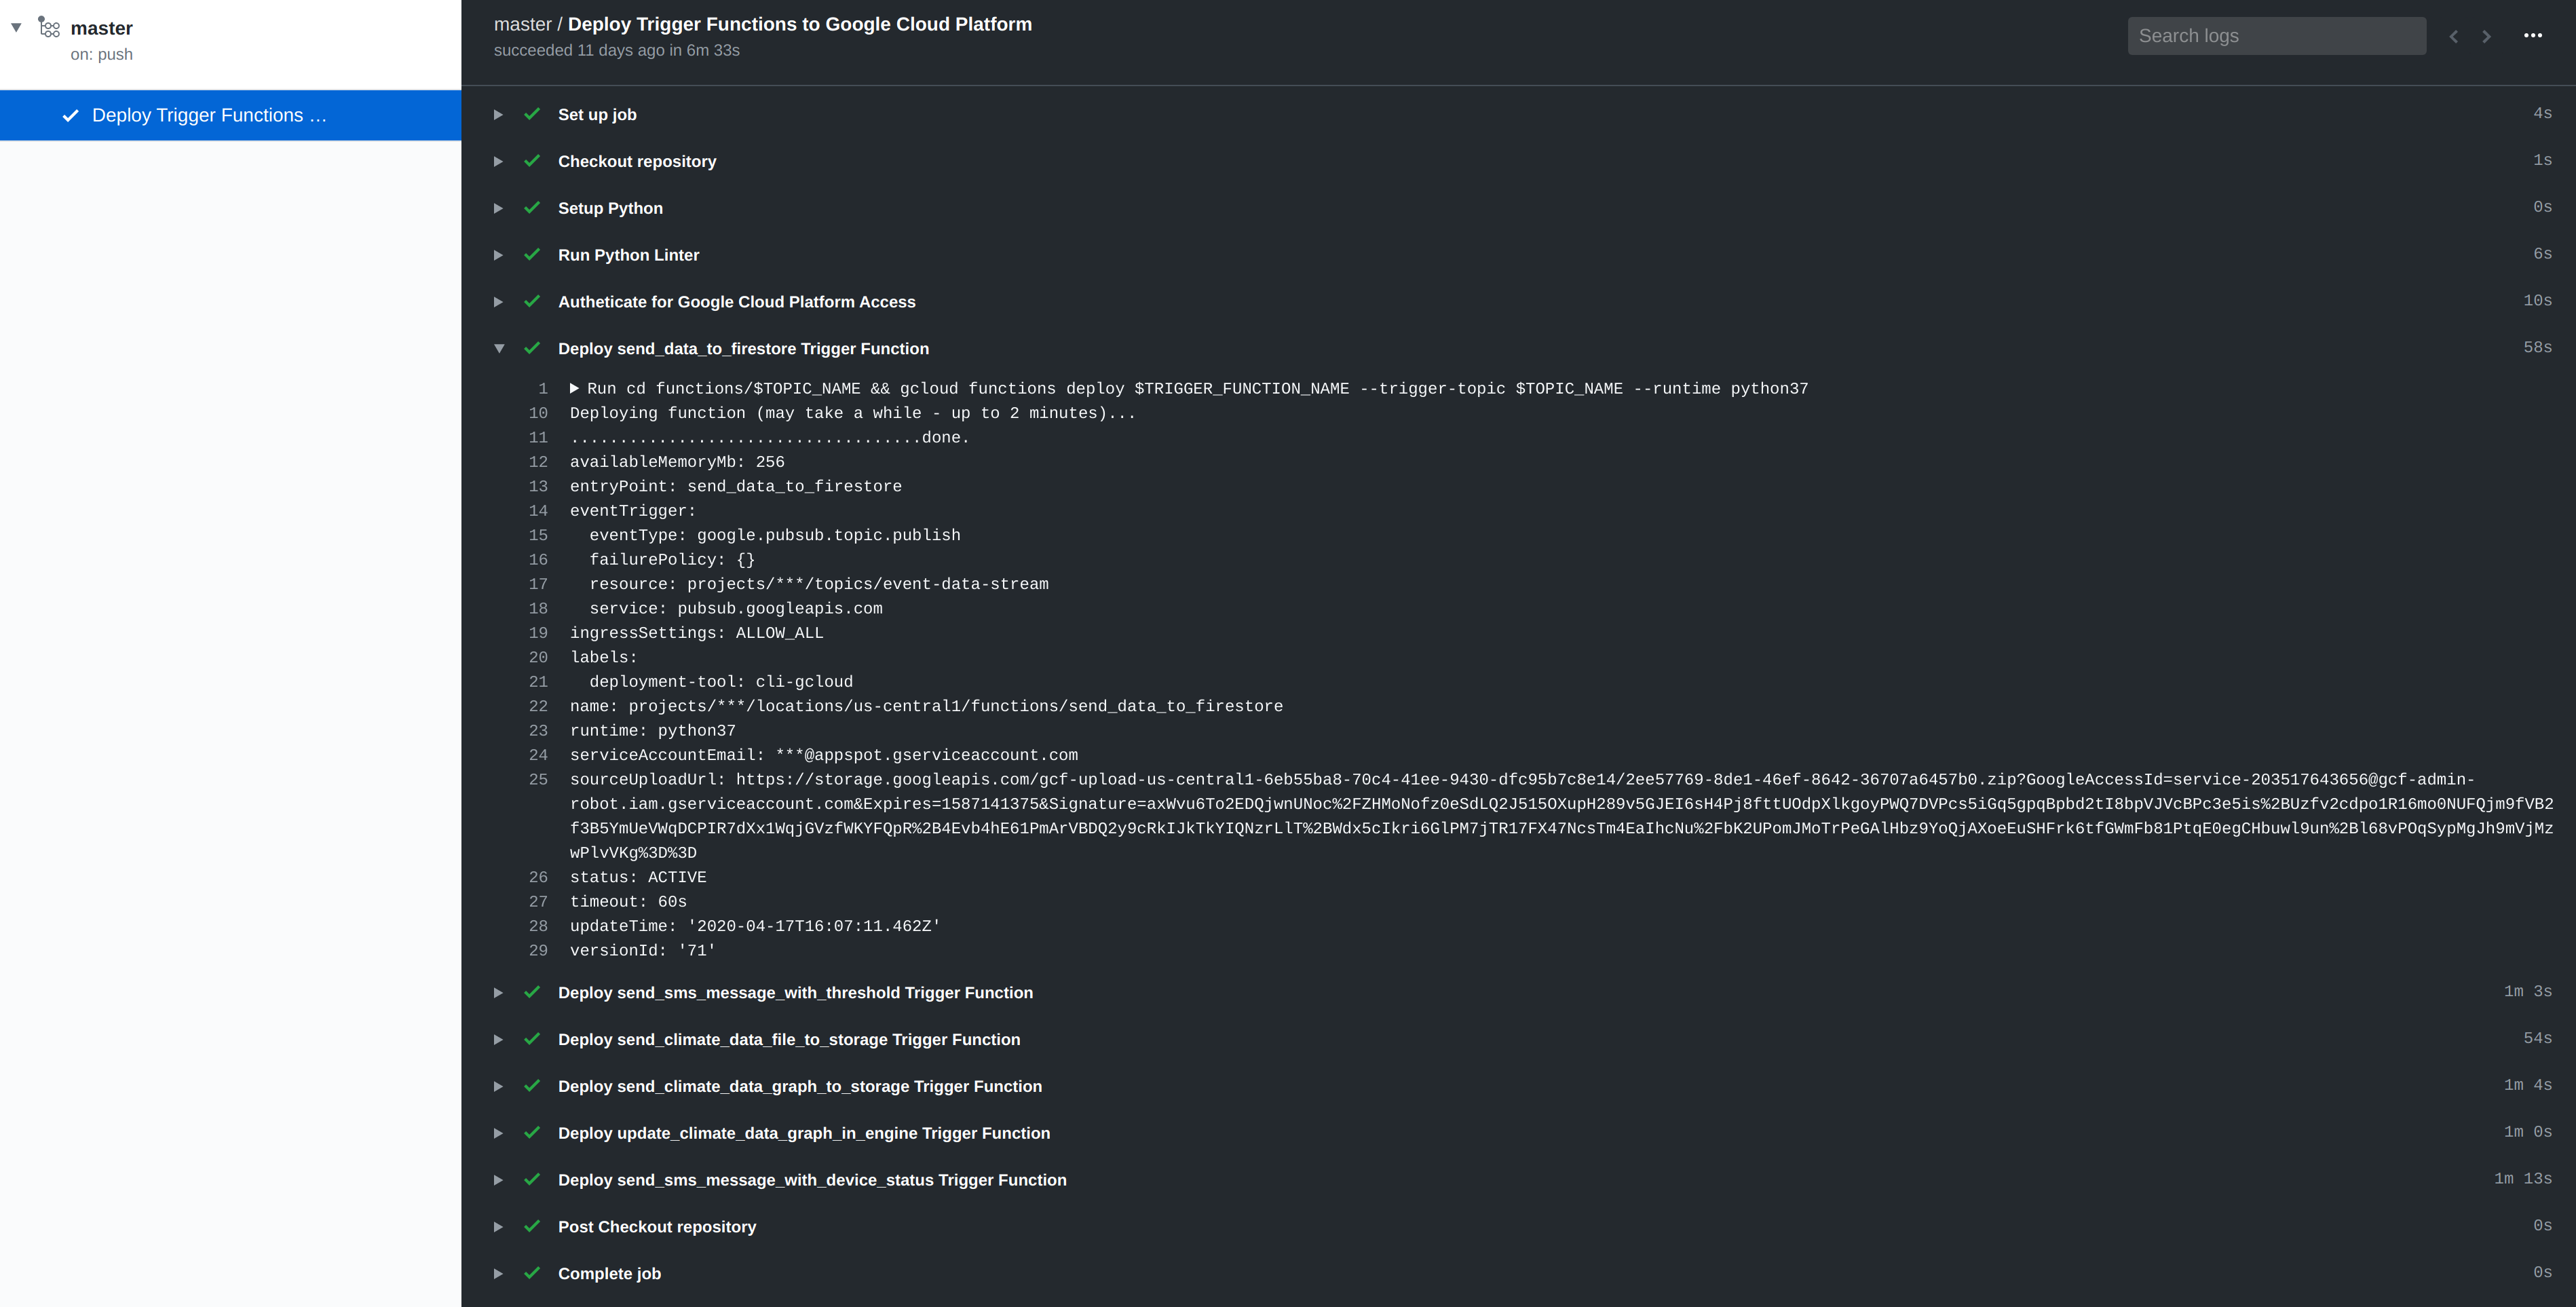
\includegraphics[width=\textwidth]{images/github-actions.png}
	\caption{GitHub Actions Workflow Visual}
	\label{fig:workflow-visual}
\end{figure}

\section{Discussion}
It was quite a difficult experience integrating all the hardware and technology stack used in the Cloud Temperature \& Humidity Notification System. This was especially true of Google Cloud Platform because while there was extensive documentation on their services, Google is a company known for renaming, rebranding, and deploying new services often. As one can imagine, that makes it difficult to discern what was changed, what to look for, and what to use. Their documentation is not very well organized as concepts and subconcepts of a particular service are scattered throughout the website. Ironically enough, it was more efficient -- though not exactly pleasant -- to Google search for what I needed than navigating through the Google Cloud Platform documentation.\\

Aside from the obvious pitfall of the documentation, Google Cloud Platform is powerful. Google manages and reduces a lot of work that would otherwise be placed as responsibility for a software engineer. As engineers, it is only natural to selectively point out aspects of a system that are nuances but truly software is a collection of reused code that makes life easier for them. Take Google Cloud functions, for example, an engineer only has to write the code to handle incoming events and Google manages the rest. The rest comprising of buying, maintaining and upgrading hardware to host servers for computational needs, developing security practices around the serverless functions, developing logging abilities on all existing functions, and the list just goes on.\\

As we are on the topic of serverless functions, I believe it is important to point out that they were the big driver behind much of the background processing necessary to create the system. A lot of the other cloud services played a role but I feel that Google Cloud Functions played the most prominent role. Serverless functions are relatively new to the software engineering field, which was popularized initially by Amazon Web Services when they released their Lambda functions in 2014. Since then it has gained traction and understandably so. Unlike the traditional approach of an always-on server -- hence the word \textit{serverless} in serverless functions -- there is very little operational overhead to speak of. I believe that this is the way of the future for software and especially IoT.\\

The results of the Cloud Temperature \& Humidity Notification System developed was possible due to the collective knowledge of many industries and intellectuals put together. That is something to be proud of and awe of when we realize how much knowledge was accumulated over time to get to this point. It is simply amazing.

\section{Conclusion}
Being able to read ambient temperature and relative humidity and send information about it can have beneficial implications when thoughtfully used. IoT -- though as vague and broad as it is, possibly even misnomer -- has large and impactful implications on humans whether; good or bad. In this case, mostly good because the system is simply reading the given environment's climate. The Cloud Temperature \& Humidity Notification System only represents an incredibly small portion of the potential of IoT.

\end{document}
